%======================================================================
\chapter{Differential equations and bifurcation}\label{ch:st}
%======================================================================

\framepart{Outline}
A system is described by a differential equation $\dot y = f(y,r)$ with a
control parameter $r$ that we turn by hand: a load, a stiffness, an
imperfection. For most values of $r$ the system has a single steady state,
and it behaves calmly. At special values of $r$ the number of steady states
changes. These are the bifurcation points. The chapter finds them and explains
why they occur exactly there: the slope $f_y = \partial f/\partial y$ at a steady
state decides both its stability and its uniqueness, and a bifurcation is the
moment the control parameter pushes this slope through zero. With several
unknowns the slope becomes the Jacobian matrix, and its eigenvalues play the same
two roles. We start from the linear equation $\dot y = ay$, which we solve
completely. We reach the buckling of a rigid bar on a spring, the first mechanical
example of the book, the galloping of a prism in the wind, and the computer
methods that follow a branch of solutions through its turning points.

\paragraph{By the end of this chapter you should be able to:}
\begin{itemize}
  \item find the steady states of $\dot y = f(y,r)$ and decide their stability
        from the sign of $f_y$, or from the eigenvalues of the Jacobian;
  \item prove stability with a Lyapunov function when the linear test is silent;
  \item locate the bifurcation points with the two conditions $f = 0$ and $f_y = 0$;
  \item recognise the fold (saddle-node), transcritical, pitchfork and Hopf
        bifurcations, draw their diagrams, and reduce a given equation to its
        normal form from a few Taylor coefficients;
  \item explain critical slowing down, imperfection sensitivity and hysteresis;
  \item compute the post-buckling path of a rigid bar from its potential energy;
  \item explain why Newton's method fails at a fold, and follow a branch through
        it by pseudo-arclength continuation.
\end{itemize}

\paragraph{Plan of the chapter.}
Section~\ref{sec:st-linear} solves the linear equation and shows what it cannot
do. Section~\ref{sec:st-slope} gives the slope test, and
Section~\ref{sec:st-lyapunov} makes stability precise with Lyapunov's two methods:
a function that decreases along the motion, and the eigenvalues of the Jacobian.
Section~\ref{sec:st-pitchfork} follows the simplest nonlinear equation in which
one solution becomes three. Section~\ref{sec:st-why} explains why this happens,
and where. Section~\ref{sec:st-normal} presents the fold, the transcritical and
the pitchfork, and shows how to reduce an equation to one of them.
Section~\ref{sec:st-hopf} adds the fourth generic bifurcation, the Hopf
bifurcation, where an oscillation is born. Section~\ref{sec:st-energy} returns to
mechanics: potential energy, the buckling bar, imperfections and hysteresis.
Section~\ref{sec:st-continuation} computes branches by continuation, and finds
that the eigenvalue problem $\mat{J}\mat{v} = \mat{0}$ decides where Newton's method
breaks down. A summary, exercises with solutions
(page~\pageref{sec:st-exo}) and the references close the chapter. The presentation follows the spirit
of~\cite{st-strang2014}: small examples solved by hand before general statements.
Many more examples are in~\cite{st-strogatz2015}; the theory is
in~\cite{st-guckenheimer1983,st-kuznetsov2004}, and the numerical side
in~\cite{st-seydel2010}.

%======================================================================
\section{Growth and decay: \texorpdfstring{$\dot y = ay$}{y' = ay}}\label{sec:st-linear}
\index{differential equation!linear}%

Start with numbers. Take $\dot y = -2y$ with $y(0) = 3$, where the dot is the
time derivative $\dot y = dy/dt$. The function $y(t) = 3e^{-2t}$ works: its
derivative is $-6e^{-2t} = -2y$, and $y(0) = 3$. After a time $t = \tfrac12$ the
value has dropped to $3/e \approx 1.10$. After $t = 2$ it is $0.055$.

The general equation and its solution are
\begin{equation}\label{eq:st-linear}
  \dot y = a\,y, \quad y(0) = y_0
  \qquad\Longrightarrow\qquad
  y(t) = y_0\,e^{at}.
\end{equation}
The number $a$ is our first control parameter, and it decides everything
(Figure~\ref{fig:st-exponentials}). If $a < 0$ the solution decays to zero,
whatever $y_0$. If $a > 0$ even a tiny $y_0$ grows without limit. If $a = 0$
nothing moves.

\begin{figure}[ht]
  \centering
  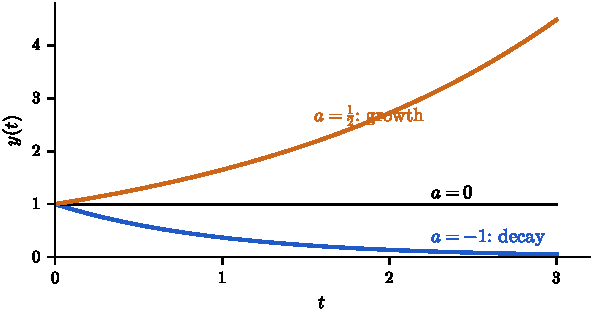
\includegraphics{ch01_bifurcation/figures/st_exponentials.pdf}
  \caption{Solutions $y = e^{at}$ of $\dot y = ay$ from $y_0 = 1$. The sign of $a$
    decides between decay and growth.}
  \label{fig:st-exponentials}
\end{figure}

\paragraph{Steady states.}
\index{steady state}%
A \emph{steady state} (or equilibrium) of $\dot y = f(y)$ is a value $y^*$ with
$f(y^*) = 0$: if we start there, we stay there. It is \emph{stable} if every
solution that starts close to $y^*$ returns to $y^*$, and \emph{unstable} if
some solutions starting arbitrarily close move away
(Section~\ref{sec:st-lyapunov} makes both words precise). For $\dot y = ay$ the only
steady state is $y^* = 0$. It is stable for $a < 0$ and unstable for $a > 0$.
The crossing $a = 0$ is where the behaviour changes.

\paragraph{A time scale.}
\index{relaxation time}%
For $a < 0$ the solution drops by the factor $e$ in the time
$\tau = 1/\abs{a}$. When $a$ is close to zero, $\tau$ is large: the system
still returns to $y = 0$, but slowly. This returns in
Section~\ref{sec:st-pitchfork} as critical slowing down.

\paragraph{What the linear equation cannot do.}
For every $a \neq 0$ the equation $ay = 0$ has one solution, $y^* = 0$. The
graph of $f(y) = ay$ is a straight line through the origin, and a straight line
crosses the axis once. However we turn the knob $a$, we never obtain two steady
states. To have several, the graph of $f$ must bend. Bifurcations need a
nonlinear $f$.

%======================================================================
\section{Steady states and the slope test}\label{sec:st-slope}
\index{stability}%

From now on $f(y)$ is any smooth function. We usually cannot solve
$\dot y = f(y)$ by a formula, and we do not need to. A picture and one
derivative tell us almost everything.

\paragraph{The phase line.}
\index{phase line}%
Draw the graph of $f(y)$ against $y$. Where $f > 0$, $\dot y > 0$ and $y$
increases: put an arrow to the right on the $y$-axis. Where $f < 0$, $y$
decreases: put an arrow to the left. The steady states are the points where
the graph crosses the axis.

\begin{example}[The logistic equation]\label{ex:st-logistic}
The equation $\dot y = y(1-y)$ models a population with limited food. Its steady
states are $y^* = 0$ and $y^* = 1$. Between them $f > 0$ and the arrows point
toward $1$. Beyond $1$, $f < 0$ and the arrows point back toward $1$. Below $0$,
$f < 0$ again and the arrows point away from $0$.
Figure~\ref{fig:st-phaseline} shows that $y^* = 1$ attracts and $y^* = 0$ repels.
We read stability without solving anything.
\end{example}

\begin{figure}[ht]
  \centering
  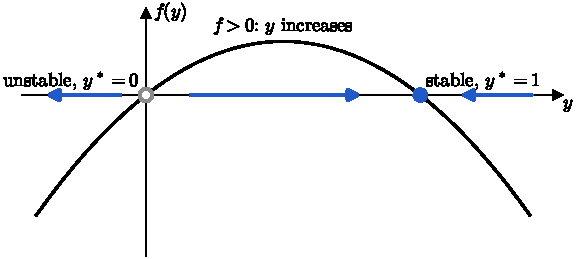
\includegraphics{ch01_bifurcation/figures/st_phaseline.pdf}
  \caption{Phase line of $\dot y = y(1-y)$. Arrows give the direction of motion.
    The filled dot is stable, the open dot unstable.}
  \label{fig:st-phaseline}
\end{figure}

At the stable state the graph of $f$ crosses the axis going down; at the
unstable one it crosses going up. ``Going down'' means $f'(y^*) < 0$.

\begin{gbox}{The slope $f'(y^*)$ is the growth rate of small disturbances}\label{sec:st-slopetest}
\index{linearization}%
Near a steady state $y^*$ of $\dot y = f(y)$, a small disturbance $\varepsilon$
obeys $\dot\varepsilon \approx \lambda\,\varepsilon$ with $\lambda = f'(y^*)$.
\begin{itemize}
  \item $\lambda < 0$: $y^*$ is stable, and disturbances decay in a time of about
        $1/\abs{\lambda}$.
  \item $\lambda > 0$: $y^*$ is unstable.
  \item $\lambda = 0$: the test is silent. The nonlinear terms decide.
\end{itemize}
\end{gbox}

\paragraph{Why it works.}
Zoom in on the crossing in Figure~\ref{fig:st-phaseline}: close enough, the
graph of $f$ is a straight line of slope $f'(y^*)$, and we are back to
Section~\ref{sec:st-linear}. In formulas, write $y = y^* + \varepsilon$. Since
$y^*$ is constant, $\dot y = \dot\varepsilon$. Taylor's formula and $f(y^*) = 0$ give
\begin{equation}\label{eq:st-linearization}
  \dot\varepsilon = f(y^* + \varepsilon)
  = f'(y^*)\,\varepsilon + O(\varepsilon^2)
  \qquad\Longrightarrow\qquad
  \varepsilon(t) \approx \varepsilon_0\,e^{\lambda t}, \quad \lambda = f'(y^*).
\end{equation}
Near every steady state, a nonlinear equation behaves like $\dot y = ay$ with
$a = f'(y^*)$.

For the logistic equation $f'(y) = 1 - 2y$, so $\lambda = 1$ at $y^* = 0$
(unstable) and $\lambda = -1$ at $y^* = 1$ (stable), as the phase line showed.

\paragraph{When the test is silent.}
The three equations $\dot y = -y^3$, $\dot y = y^3$ and $\dot y = y^2$ all have
$y^* = 0$ with $\lambda = 0$. The first is stable, the second unstable, and the
third attracts from the left and repels to the right. When $\lambda = 0$ the
linear approximation has thrown away exactly the information we need. This is
not an accident: $\lambda = 0$ is where bifurcations happen.

%======================================================================
\section{Lyapunov stability}\label{sec:st-lyapunov}
\index{stability!Lyapunov}%

The slope test looks at a steady state through a magnifying glass. Two questions
remain. What exactly does ``stable'' mean? And what do we do when the glass shows
nothing ($\lambda = 0$), or when there are several unknowns? Lyapunov answered both
in 1892~\cite{st-lyapunov1992}, with two methods. The first uses a function that
decreases along the motion. The second uses the eigenvalues of a matrix.

\paragraph{Two definitions.}
Let $y^*$ be a steady state of $\dot y = f(y)$, where $y$ may now be a column of
$n$ unknowns and $\abs{\cdot}$ its length.
\begin{itemize}
  \item $y^*$ is \emph{stable} (in the sense of Lyapunov) if solutions that start
        close stay close: for every distance $\varepsilon > 0$ there is a
        $\delta > 0$ such that $\abs{y(0) - y^*} < \delta$ implies
        $\abs{y(t) - y^*} < \varepsilon$ for all $t \ge 0$.
  \item $y^*$ is \emph{asymptotically stable} if it is stable and, in addition,
        $y(t) \to y^*$ for every start close enough.
\end{itemize}
A frictionless pendulum hanging down is stable but not asymptotically stable: a
small push gives a small swing that never dies. Add friction and the swing dies
out. In Section~\ref{sec:st-slope}, $\lambda < 0$ gave asymptotic stability. For
the equilibria of conservative structures, Lyapunov's first definition is the
natural one (Chapter~\ref{ch:ld}).

\begin{gbox}{A function that decreases along every motion proves stability}\label{sec:st-lyapdirect}
\index{Lyapunov function}%
Let $W(y)$ have a strict minimum at $y^*$: $W(y^*) = 0$ and $W(y) > 0$ for
$y \neq y^*$ near $y^*$. Along a solution of $\dot y = f(y)$, $W$ changes at the rate
$\dot W = \nabla W \cdot f(y)$.
\begin{itemize}
  \item If $\dot W \le 0$ near $y^*$, then $y^*$ is stable.
  \item If $\dot W < 0$ near $y^*$, except at $y^*$ itself, then $y^*$ is
        asymptotically stable.
\end{itemize}
Such a $W$ is a \emph{Lyapunov function}. No solution of the equation is needed.
\end{gbox}

\paragraph{Why it works.}
Picture the level curves $W = \text{const}$ around $y^*$ as nested bowls
(Figure~\ref{fig:st-lyapunov}). Since $W$ never increases, a solution can never
climb from one level to a higher one. Start inside a small level curve and you stay
inside it: that is stability. If $W$ strictly decreases, the solution keeps going
down until it reaches the bottom $W = 0$, which is $y^*$.

\paragraph{When the slope test is silent.}
Take $\dot y = -y^3$ and $W = \tfrac12 y^2$. Then
$\dot W = y\,\dot y = -y^4 < 0$ for $y \neq 0$: the origin is asymptotically
stable. For $\dot y = y^3$ the same $W$ gives $\dot W = +y^4$, and the origin is
unstable. One well-chosen function settles what the linear approximation could not.

\paragraph{The damped oscillator.}
\index{oscillator!damped}%
A mass $m$ on a spring $k$ with a dashpot $c$ obeys $m\ddot x + c\dot x + kx = 0$.
There are two unknowns, the position $x$ and the velocity $\dot x$, and the rest
state is $(x,\dot x) = (0,0)$. Take for $W$ the mechanical energy
\begin{equation}\label{eq:st-energy-osc}
  E = \frac12\,m\,\dot x^2 + \frac12\,k\,x^2 .
\end{equation}
Along a motion,
\begin{equation}\label{eq:st-energy-rate}
  \dot E = m\,\dot x\,\ddot x + k\,x\,\dot x
  = \dot x\,(m\ddot x + kx) = -c\,\dot x^2 \le 0 .
\end{equation}
The dashpot only takes energy away, so the rest state is stable. Here $\dot E = 0$
on the whole line $\dot x = 0$, not only at the origin, and the second bullet does
not apply as stated. But a motion cannot stay on that line unless $x = 0$: away from
the origin the spring pushes the mass off it. So the energy keeps decreasing and the
rest state is asymptotically stable (this refinement is due to LaSalle). With
$c = 0$ the energy is constant: stable, not asymptotically stable, as for the
frictionless pendulum.

\begin{figure}[ht]
  \centering
  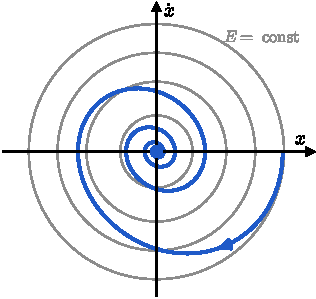
\includegraphics{ch01_bifurcation/figures/st_lyapunov.pdf}
  \caption{A motion of the damped oscillator ($m = k = 1$, $c = 0.3$) crosses the
    level curves of the energy $E$ inward, and never outward. The energy is a
    Lyapunov function.}
  \label{fig:st-lyapunov}
\end{figure}

\paragraph{Energy is the Lyapunov function of mechanics.}
For a conservative structure the total energy, kinetic plus potential, is constant.
If the potential energy has a strict minimum at an equilibrium, the total energy is a
Lyapunov function, and the equilibrium is stable. This is the theorem of
Lagrange and Dirichlet. It is the basis of the energy criterion of
Chapter~\ref{ch:ld}, and it is why buckling problems can be solved without ever
writing the equations of motion.
\index{Lagrange--Dirichlet theorem}%

\paragraph{Several unknowns: the Jacobian.}
\index{Jacobian matrix}%
For $n$ unknowns we write the state as a column $\mat{y}$ and the equation as
$\dot{\mat{y}} = \mat{f}(\mat{y})$. Near a steady state $\mat{y}^*$, a small
disturbance $\boldsymbol{\varepsilon}$ obeys $\dot{\boldsymbol{\varepsilon}} = \mat{J}\boldsymbol{\varepsilon}$,
where the \emph{Jacobian} $\mat{J}$ is the $n\times n$ matrix of the slopes
$J_{ij} = \partial f_i/\partial y_j$ at $\mat{y}^*$. When $\mat{J}$ has $n$
independent eigenvectors $\mat{x}_i$ with eigenvalues $\lambda_i$,
\begin{equation}\label{eq:st-modes}
  \boldsymbol{\varepsilon}(t) = c_1\,e^{\lambda_1 t}\,\mat{x}_1 + \dots
  + c_n\,e^{\lambda_n t}\,\mat{x}_n .
\end{equation}
Each eigenvalue is a growth rate, as $f'(y^*)$ was. A complex pair
$\lambda = \alpha \pm i\omega$ gives
$e^{\lambda t} = e^{\alpha t}(\cos\omega t \pm i\sin\omega t)$: an oscillation of
frequency $\omega$ whose amplitude grows or decays at the rate $\alpha$.

\begin{gbox}{The eigenvalues of the Jacobian are the growth rates of disturbances}\label{sec:st-eigen}
\index{stability!eigenvalues}%
Let $\lambda_1,\dots,\lambda_n$ be the eigenvalues of $\mat{J}$ at the steady state
$\mat{y}^*$.
\begin{itemize}
  \item All real parts negative: $\mat{y}^*$ is asymptotically stable.
  \item One real part positive: $\mat{y}^*$ is unstable.
  \item Some real parts zero, none positive: the test is silent.
\end{itemize}
\end{gbox}

\paragraph{Why it works.}
Close to $\mat{y}^*$ the neglected terms are of order $\abs{\boldsymbol{\varepsilon}}^2$,
too small to compete with an exponential. Lyapunov's own proof is a bridge between
his two methods: from $\mat{J}$ he builds a quadratic Lyapunov function
$W = \boldsymbol{\varepsilon}\T\mat{P}\boldsymbol{\varepsilon}$
(details in~\cite{st-guckenheimer1983}). The slope test of
Section~\ref{sec:st-slopetest} is the case $n = 1$.

\begin{example}[Eigenvalues of the damped oscillator]\label{ex:st-osc-eig}
With $m = 1$, $c = 3$, $k = 2$ the oscillator becomes, for $\mat{y} = (x,\dot x)$,
\[
  \frac{d}{dt}\begin{bmatrix} x\\ \dot x\end{bmatrix}
  = \begin{bmatrix} 0 & 1\\ -2 & -3\end{bmatrix}
    \begin{bmatrix} x\\ \dot x\end{bmatrix},
  \qquad
  \det(\mat{J} - \lambda\mat{I}) = \lambda^2 + 3\lambda + 2 = (\lambda+1)(\lambda+2).
\]
The eigenvalues $-1$ and $-2$ are negative: the rest state is stable and the mass
creeps back without oscillating. With $c = 1$ instead, $\lambda^2 + \lambda + 2 = 0$
gives $\lambda = -\tfrac12 \pm i\,\tfrac{\sqrt7}{2}$: a decaying oscillation.
In general $\lambda^2 + (c/m)\lambda + k/m = 0$.
\end{example}

\paragraph{Two ways to lose stability.}
\index{divergence}\index{flutter}%
For two unknowns the eigenvalues solve
$\lambda^2 - (\tr\mat{J})\,\lambda + \det\mat{J} = 0$, so
$\lambda_1 + \lambda_2 = \tr\mat{J}$ and $\lambda_1\lambda_2 = \det\mat{J}$. Both
real parts are negative exactly when $\tr\mat{J} < 0$ and $\det\mat{J} > 0$
(Figure~\ref{fig:st-tracedet}). A parameter that drives the system out of this
quarter plane must cross one of its two edges.
\begin{itemize}
  \item $\det\mat{J}$ reaches zero: one real eigenvalue passes through $0$. The
        structure moves away without oscillating. This is \emph{divergence}, the
        static loss of stability, and buckling is the example. Put a mass $m$ on top
        of the bar of Section~\ref{sec:st-energy}:
        $mL^2\ddot\theta + c\dot\theta + k\theta - PL\sin\theta = 0$. At $\theta = 0$,
        $\det\mat{J} = (k - PL)/(mL^2)$, which vanishes at the critical load
        $P_c = k/L$, while $\tr\mat{J} = -c/(mL^2)$ does not change.
  \item $\tr\mat{J}$ reaches zero while $\det\mat{J} > 0$: a pair $\pm i\omega$
        crosses the imaginary axis. The structure oscillates with a growing
        amplitude: the damping has become negative. This is \emph{flutter} or
        \emph{galloping}, the dynamic loss of stability (Section~\ref{sec:st-hopf}).
\end{itemize}
Both happen in practice, and they need different analyses: the first only the
stiffness, the second also the mass and the damping.

\begin{figure}[ht]
  \centering
  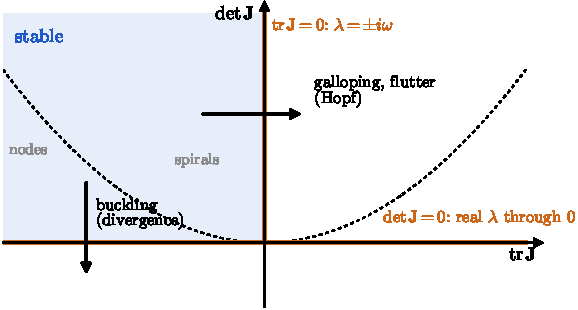
\includegraphics{ch01_bifurcation/figures/st_tracedet.pdf}
  \caption{Stability of a $2\times2$ Jacobian. The shaded quarter plane is stable.
    Crossing $\det\mat{J} = 0$ is divergence (buckling); crossing
    $\tr\mat{J} = 0$ with $\det\mat{J} > 0$ is a Hopf bifurcation (galloping,
    flutter). Above the dotted parabola $(\tr\mat{J})^2 = 4\det\mat{J}$ the
    eigenvalues are complex.}
  \label{fig:st-tracedet}
\end{figure}

%======================================================================
\section{The pitchfork: one solution becomes three}\label{sec:st-pitchfork}
\index{bifurcation!pitchfork}%

Here is the simplest equation in which the number of steady states changes as
we turn a parameter:
\begin{equation}\label{eq:st-pitchfork}
  \dot y = f(y,r) = r\,y - y^3 .
\end{equation}
The right side has two competing terms. The linear term $ry$ is the equation of
Section~\ref{sec:st-linear}: it pulls $y$ back toward zero when $r < 0$ and pushes
it away when $r > 0$. The cubic term $-y^3$ always pulls back, and for large
$\abs{y}$ it wins. It keeps the solutions from running off to infinity.

\paragraph{Steady states.}
Set $f = 0$ and factor: $ry - y^3 = y\,(r - y^2) = 0$. Either $y = 0$, or
$y^2 = r$, which has the two real roots $y = \pm\sqrt r$ only when $r > 0$.
There is one steady state for $r \le 0$ and three for $r > 0$.

\paragraph{Stability.}
The slope is $f_y = r - 3y^2$. On each branch:
\begin{center}
\begin{tabular}{@{}llll@{}}
  \toprule
  steady state & exists for & $\lambda = f_y(y^*,r)$ & stability \\
  \midrule
  $y^* = 0$         & all $r$ & $r$           & stable if $r < 0$, unstable if $r > 0$ \\
  $y^* = \pm\sqrt r$ & $r > 0$ & $r - 3r = -2r$ & stable \\
  \bottomrule
\end{tabular}
\end{center}

\paragraph{The story as $r$ increases.}
For $r < 0$ there is one steady state, $y = 0$, and it attracts everything.
As $r$ rises to $0$, the growth rate $\lambda = r$ at the origin rises to zero.
For $r > 0$ the origin is still a steady state, but an unstable one, and two new
stable states $\pm\sqrt r$ have appeared on either side.
Figure~\ref{fig:st-pitchfork} draws the steady states against the control
parameter. This picture is the \emph{bifurcation diagram}, and its shape gives
the bifurcation its name.
\index{bifurcation!diagram}%

\begin{figure}[ht]
  \centering
  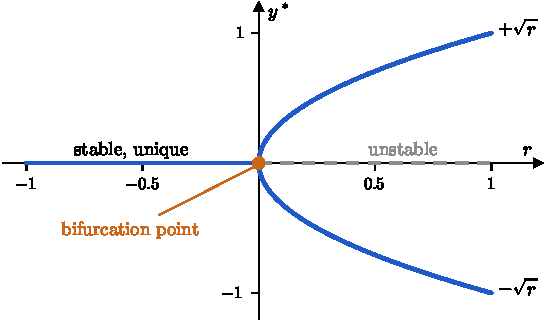
\includegraphics{ch01_bifurcation/figures/st_pitchfork.pdf}
  \caption{Bifurcation diagram of $\dot y = ry - y^3$. Solid: stable steady
    states. Dashed: unstable. At $r = 0$ one branch splits into three.}
  \label{fig:st-pitchfork}
\end{figure}

\paragraph{Symmetry breaking.}
\index{symmetry breaking}%
Equation~\eqref{eq:st-pitchfork} is unchanged when $y$ is replaced by $-y$. It
has no preference for left or right. Yet for $r > 0$ the system must settle at
$+\sqrt r$ or at $-\sqrt r$, and each of these does prefer a side. The choice is
made by the small disturbance that first pushed $y$ away from zero. The law is
symmetric; the outcome is not.

\begin{gbox}{Near a bifurcation, the system recovers more and more slowly}\label{sec:st-slowing}
\index{critical slowing down}%
For $r < 0$ disturbances of $y^* = 0$ decay in the time $\tau = 1/\abs{r}$, which
grows without limit as $r \to 0$. At $r = 0$ the decay is no longer exponential:
\begin{equation}\label{eq:st-slowdecay}
  \dot y = -y^3, \quad y(0) = y_0
  \qquad\Longrightarrow\qquad
  y(t) = \frac{y_0}{\sqrt{1 + 2y_0^2\,t}} \sim \frac{1}{\sqrt{2t}} .
\end{equation}
\end{gbox}

\paragraph{Why it works.}
The first statement is the slope test of Section~\ref{sec:st-slopetest} with
$\lambda = r$. At $r = 0$ the valley around $y = 0$ becomes flat, and a flat
valley drains slowly. Separate the variables in $\dot y = -y^3$:
\[
  \frac{dy}{y^3} = -\,dt
  \quad\Longrightarrow\quad
  \frac{1}{2y^2} = t + \frac{1}{2y_0^2}
  \quad\Longrightarrow\quad
  \frac{1}{y^2} = \frac{1}{y_0^2} + 2t ,
\]
which is~\eqref{eq:st-slowdecay}. The decay like $1/\sqrt t$ is far slower than
any exponential. In experiments, and in the records of ecosystems and the
climate~\cite{st-scheffer2009}, this slowing down is often the first visible
warning that a bifurcation is near. Exercise~\ref{exo:st-computer-pitchfork}
measures it numerically.

%======================================================================
\section{Why bifurcations happen}\label{sec:st-why}
\index{bifurcation!point}%

We have watched one solution become three. Now we explain it. Suppose $y^*$ is a
steady state at the parameter value $r$, so $f(y^*,r) = 0$. Change $r$ by a small
amount $\Delta r$. The steady state moves to $y^* + \Delta y$, and it must still
satisfy $f = 0$. To first order,
\begin{equation}\label{eq:st-ift}
  f_y\,\Delta y + f_r\,\Delta r = 0
  \qquad\Longrightarrow\qquad
  \Delta y = -\frac{f_r}{f_y}\,\Delta r .
\end{equation}
If $f_y \neq 0$, this has exactly one answer $\Delta y$: the steady state follows
the parameter along a single smooth curve, like a bead on a wire, and no new
branch can leave it. If $f_y = 0$, we divide by zero. The first-order equation no
longer fixes $\Delta y$, and the higher-order terms decide how many solutions
there are.

\begin{gbox}{New steady states can appear only where $f = 0$ and $f_y = 0$}\label{sec:st-ift}
\index{implicit function theorem}%
If $f(y_0,r_0) = 0$ and $f_y(y_0,r_0) \neq 0$, then for $r$ close to $r_0$ there
is exactly one steady state $y^*(r)$ close to $y_0$. It depends smoothly on $r$,
and $\displaystyle\frac{dy^*}{dr} = -\frac{f_r}{f_y}$. The number of steady states
can therefore change only at a point where
\begin{equation}\label{eq:st-bifcondition}
  f(y_0,r_0) = 0 \qquad\text{and}\qquad f_y(y_0,r_0) = 0 .
\end{equation}
\end{gbox}

\paragraph{Why it works.}
Picture the curve $f(y,r) = 0$ in the $(r,y)$ plane: it is the bifurcation
diagram. Where $f_y \neq 0$ the curve is the graph of a function $y^*(r)$, with
the slope~\eqref{eq:st-ift}, and a vertical line $r = \text{const}$ meets it once
nearby. Branches can meet, split or turn back only where this slope is
infinite or undefined, that is where $f_y = 0$. This is the implicit function
theorem in one variable; Figure~\ref{fig:st-ift} draws it, and
Section~\ref{sec:st-iftn} states it for several unknowns.

\paragraph{One number, two jobs.}
The number $f_y(y^*,r)$ was the growth rate $\lambda$ in
Section~\ref{sec:st-slopetest}: it decides \emph{stability}. Here it is the
denominator: it decides \emph{uniqueness}. So a steady state can lose its
uniqueness only at the moment it loses (or gains) stability. As the control
parameter pushes $\lambda$ from negative to positive, it must pass through
$\lambda = 0$, and at that instant new steady states are free to appear. This is
the answer to the question of the chapter.

\paragraph{Check on the pitchfork.}
With $f = ry - y^3$ we have $f_y = r - 3y^2$ and $f_r = y$. The two conditions
$f = 0$ and $f_y = 0$ hold together only at $(y,r) = (0,0)$, the single
bifurcation point of Figure~\ref{fig:st-pitchfork}. On the upper branch
$y^* = \sqrt r$ the slope formula gives
$\displaystyle\frac{dy^*}{dr} = -\frac{\sqrt r}{-2r} = \frac{1}{2\sqrt r}$, the
derivative of $\sqrt r$, as it should. It blows up as $r \to 0$: the branch leaves
the bifurcation point vertically, because $f_y \to 0$ there.

\paragraph{Several unknowns.}
For $\dot{\mat{y}} = \mat{f}(\mat{y},r)$ with $n$ unknowns the first-order
equation~\eqref{eq:st-ift} becomes
\begin{equation}\label{eq:st-iftn}
  \mat{J}\,\Delta\mat{y} + \mat{f}_r\,\Delta r = \mat{0},
\end{equation}
where $\mat{f}_r$ is the column $\partial\mat{f}/\partial r$. If $\mat{J}$ is
invertible, $\Delta\mat{y} = -\mat{J}^{-1}\mat{f}_r\,\Delta r$ and the steady state
moves along a single smooth branch. The first-order argument is made exact by the
implicit function theorem.

\begin{gbox}{The implicit function theorem: an invertible Jacobian gives one smooth branch}\label{sec:st-iftn}
\index{implicit function theorem}%
Let $\mat{f}(\mat{y},r)$, with $n$ unknowns $\mat{y}$ and one parameter $r$, have
continuous first derivatives. Suppose that at the point $(\mat{y}_0,r_0)$
\begin{equation}\label{eq:st-iftcond}
  \mat{f}(\mat{y}_0,r_0) = \mat{0}
  \qquad\text{and}\qquad
  \det\mat{J}(\mat{y}_0,r_0) \neq 0 .
\end{equation}
Then there is a box around the point, an interval $I$ around $r_0$ times a
neighbourhood $V$ of $\mat{y}_0$, in which the solutions of $\mat{f} = \mat{0}$ are
exactly the graph of one function $\mat{y}^*(r)$: for $r$ in $I$ and $\mat{y}$ in
$V$,
\begin{equation}\label{eq:st-iftgraph}
  \mat{f}(\mat{y},r) = \mat{0}
  \quad\Longleftrightarrow\quad
  \mat{y} = \mat{y}^*(r).
\end{equation}
The function $\mat{y}^*$ has continuous derivatives, and
$\displaystyle\frac{d\mat{y}^*}{dr} = -\mat{J}^{-1}\mat{f}_r$.
\end{gbox}

\paragraph{Why it works.}
Look at the left panel of Figure~\ref{fig:st-ift}. Inside the small box, every
vertical line $r = \text{const}$ meets the solution curve exactly once, so the
curve is a graph over $r$. In formulas, freeze $r$ in $I$ and iterate the Newton
step with the fixed matrix $\mat{J}_0 = \mat{J}(\mat{y}_0,r_0)$:
\[
  \mat{y} \leftarrow \mat{y} - \mat{J}_0^{-1}\mat{f}(\mat{y},r).
\]
Since $\mat{J}_0$ is invertible and the derivatives are continuous, the box can be
made so small that each step shrinks distances by a factor less than one. The
iteration then converges to exactly one $\mat{y}$ in $V$: this is $\mat{y}^*(r)$.
Differentiating $\mat{f}(\mat{y}^*(r),r) = \mat{0}$ gives
$\mat{J}\,d\mat{y}^*/dr + \mat{f}_r = \mat{0}$, the slope. The complete proof is in
Rudin~\cite[Theorem~9.28]{st-rudin1976}; the many forms of the theorem, and its
history from Newton and Lagrange to numerical homotopy methods, are
in~\cite{st-krantz2002}.

\paragraph{Its twin, the inverse function theorem.}
\index{inverse function theorem}%
A map $\mat{g}$ from $\R^n$ to $\R^n$ whose Jacobian is invertible at a point
$\mat{a}$ has, near $\mat{a}$, a smooth inverse, and the Jacobian of the inverse is
the inverse of the Jacobian~\cite[Theorem~9.24]{st-rudin1976}. The two theorems are
one: apply the inverse function theorem to the map
$(\mat{y},r) \mapsto (\mat{f}(\mat{y},r),\,r)$, whose Jacobian
$\begin{bmatrix}\mat{J} & \mat{f}_r\\ \mat{0}\T & 1\end{bmatrix}$ is invertible
exactly when $\mat{J}$ is.

\paragraph{The circle: what the theorem does not say.}
Take $f(y,r) = r^2 + y^2 - 1$, the unit circle (Figure~\ref{fig:st-ift}). Here
$f_y = 2y$ and $f_r = 2r$. Wherever $y \neq 0$ the theorem gives a branch,
$y^* = \sqrt{1 - r^2}$ or $-\sqrt{1 - r^2}$. At $(1,0)$, $f_y = 0$. The circle is
still a perfectly smooth curve there, but its tangent is vertical: every vertical
line near $r = 1$ meets it twice or not at all, and no box makes it a graph over
$r$. This is a fold, and it fails the test only because we chose $r$ as the
variable. Since $f_r = 2 \neq 0$, the theorem applies with the roles exchanged:
near $(1,0)$, $r$ is a function of $y$, $r^* = \sqrt{1 - y^2}$. At a branch point
(right panel) both $f_y$ and $f_r$ vanish: two curves cross, and no choice of
variable makes the solution set a graph. Section~\ref{sec:st-continuation} turns
this remark into a method: let the curve choose its own variable.

\begin{figure}[ht]
  \centering
  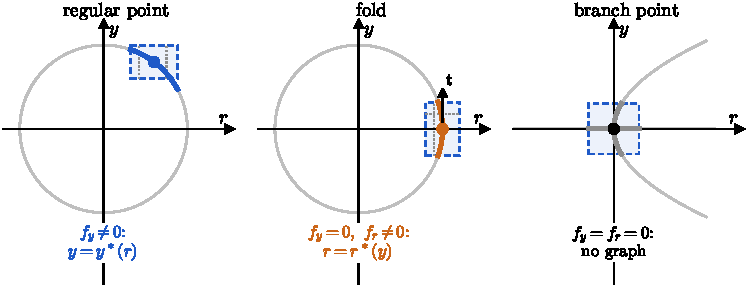
\includegraphics{ch01_bifurcation/figures/st_ift.pdf}
  \caption{The implicit function theorem in pictures. Left: at a regular point of the
    circle $r^2 + y^2 = 1$ ($f_y \neq 0$) the solutions inside a small box form the
    graph of $y^*(r)$. Middle: at the fold $(1,0)$, $f_y = 0$ and no box gives a graph
    over $r$, but $f_r \neq 0$ and the curve is the graph of $r^*(y)$; the tangent
    $\mathbf{t}$ is vertical. Right: at the branch point of the pitchfork
    $ry - y^3 = 0$, $f_y = f_r = 0$ and two curves cross: no graph in any direction.}
  \label{fig:st-ift}
\end{figure}

\paragraph{The singular case.}
The theorem can fail only where $\det\mat{J} = 0$, the form that $f_y = 0$
takes with $n$ unknowns: the Jacobian has a zero eigenvalue,
\begin{equation}\label{eq:st-zeroeig}
  \mat{J}\,\mat{v} = \mat{0}, \qquad \mat{w}\T\mat{J} = \mat{0}\T .
\end{equation}
The right eigenvector $\mat{v}$ and the left eigenvector $\mat{w}$ (an eigenvector
of $\mat{J}\T$) decide what happens next.

\begin{gbox}{Branches meet only where the Jacobian has a zero eigenvalue}\label{sec:st-zero}
\index{bifurcation!point}\index{Jacobian matrix!zero eigenvalue}%
At a steady state where $\mat{J}\mat{v} = \mat{0}$ and $\mat{w}\T\mat{J} = \mat{0}\T$
for a simple zero eigenvalue:
\begin{itemize}
  \item if $\mat{w}\T\mat{f}_r \neq 0$, the branch turns back in the direction
        $\mat{v}$: a \emph{fold};
  \item if $\mat{w}\T\mat{f}_r = 0$, a second branch can cross: a \emph{branch point}
        (transcritical or pitchfork).
\end{itemize}
In both cases $\mat{v}$ is the shape of the change. In buckling it is the
\emph{buckling mode}.
\end{gbox}

\paragraph{Why it works.}
Multiply~\eqref{eq:st-iftn} on the left by $\mat{w}\T$. Since
$\mat{w}\T\mat{J} = \mat{0}\T$, what remains is $(\mat{w}\T\mat{f}_r)\,\Delta r = 0$.
If $\mat{w}\T\mat{f}_r \neq 0$, then $\Delta r = 0$ to first order and
$\mat{J}\Delta\mat{y} = \mat{0}$, so $\Delta\mat{y} = a\,\mat{v}$: the branch has a
``vertical'' tangent, the parameter stops increasing, and the branch turns back.
If $\mat{w}\T\mat{f}_r = 0$, every $\Delta r$ is allowed and
$\Delta\mat{y} = \Delta\mat{y}_0\,\Delta r + a\,\mat{v}$ contains a free amplitude
$a$: the first order no longer picks one branch, and the second-order terms decide
how many pass through the point. In one dimension $\mat{w} = \mat{v} = 1$ and the
test reads: fold if $f_r \neq 0$, branch point if $f_r = 0$, as in
Section~\ref{sec:st-normal}.

\paragraph{The other way to lose stability.}
A complex pair $\pm i\omega$ on the imaginary axis leaves $\mat{J}$ invertible
(for $n = 2$, $\det\mat{J} = \omega^2 > 0$). The steady state goes on smoothly and
no new steady state appears. What appears instead is a periodic motion:
Section~\ref{sec:st-hopf}.

\begin{gbox}{Box 1.1\quad Finding the bifurcation points of $\dot y = f(y,r)$}\label{sec:st-box-bif}
\index{bifurcation!point}%
\begin{enumerate}[label=\arabic*.]
  \item Solve $f(y,r) = 0$ for the branches of steady states $y^*(r)$.
  \item On each branch compute $\lambda = f_y(y^*,r)$. Its sign gives stability.
  \item Find where $\lambda = 0$ (with $n$ unknowns, where $\det\mat{J} = 0$).
        These points are the only candidates.
  \item At each candidate, look at $f_r$ and at the next derivatives of $f$ to
        decide the type of bifurcation (Section~\ref{sec:st-normal}).
\end{enumerate}
\end{gbox}

%======================================================================
\section{Fold, transcritical and pitchfork: normal forms}\label{sec:st-normal}
\index{bifurcation!normal form}%

The two conditions $f = f_y = 0$ can be met in different ways. Each way has a
simplest representative, its \emph{normal form}. Near a bifurcation point, a
more complicated $f$ behaves like one of these three, and a few of its derivatives
tell which.

\begin{center}
\begin{tabular}{@{}llll@{}}
  \toprule
  type & normal form & steady states & at $r = 0$ \\
  \midrule
  saddle-node   & $\dot y = r + y^2$  & $\pm\sqrt{-r}$ for $r < 0$, none for $r > 0$ & two collide and vanish \\
  transcritical & $\dot y = ry - y^2$ & $0$ and $r$, for all $r$                    & two cross, swap stability \\
  pitchfork     & $\dot y = ry - y^3$ & $0$; and $\pm\sqrt r$ for $r > 0$           & one splits into three \\
  \bottomrule
\end{tabular}
\end{center}

\paragraph{Saddle-node.}
\index{bifurcation!saddle-node}\index{bifurcation!fold}%
For $\dot y = r + y^2$ the steady states solve $y^2 = -r$. When $r < 0$ there are
two, $y^* = \pm\sqrt{-r}$. The slope is $f_y = 2y$, so the lower one is stable
and the upper one is unstable. As $r$ increases to $0$ they meet at $y = 0$ and
disappear. For $r > 0$, $f > 0$ everywhere: there is no steady state, and $y$
runs away. The count goes $2 \to 1 \to 0$. This is the most common way a real
system fails suddenly. The point is also called a \emph{fold}, because the branch
folds back on itself, and in structural mechanics a \emph{limit point}: the load
reaches a maximum there.

\paragraph{Transcritical.}
\index{bifurcation!transcritical}%
For $\dot y = ry - y^2 = y(r - y)$ the steady states are $y^* = 0$ and $y^* = r$
for every $r$. The slope is $f_y = r - 2y$: it equals $r$ at $y^* = 0$ and $-r$
at $y^* = r$. The two branches cross at $r = 0$ and exchange stability
(Figure~\ref{fig:st-normalforms}).

\begin{figure}[ht]
  \centering
  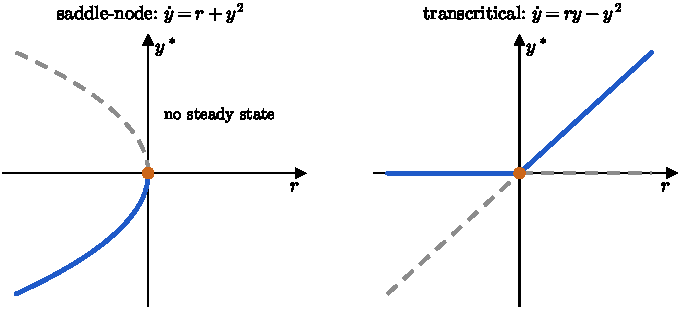
\includegraphics{ch01_bifurcation/figures/st_normalforms.pdf}
  \caption{Bifurcation diagrams of the saddle-node and transcritical normal forms.
    Solid: stable. Dashed: unstable.}
  \label{fig:st-normalforms}
\end{figure}

\paragraph{Telling them apart.}
All three have $f = f_y = 0$ at the origin. Look at $f_r$. In the saddle-node,
$f_r = 1 \neq 0$: changing $r$ moves the graph of $f$ up or down and pushes two
roots together. In the transcritical and pitchfork cases, $f_r = y = 0$ at the
point, because $y = 0$ is a steady state for every $r$. Such a persistent state
is usually forced by the physics (an unloaded state, a straight column) or by a symmetry.
The pitchfork needs, in addition, the symmetry $y \to -y$ that kills the $y^2$ term.

\paragraph{From any $f$ to its normal form.}
\index{bifurcation!normal form}%
Let $(y_0,r_0)$ be a bifurcation point, $f = f_y = 0$. Write $y = y_0 + u$,
$r = r_0 + \mu$ and expand $f$ in a Taylor series, all derivatives taken at the
point:
\begin{equation}\label{eq:st-taylor}
  \dot u = f_r\,\mu + \frac12 f_{yy}\,u^2 + f_{yr}\,u\,\mu
  + \frac12 f_{rr}\,\mu^2 + \frac16 f_{yyy}\,u^3 + \dots
\end{equation}
Near the point only the largest terms matter. Which ones they are depends on which
coefficients vanish.
\begin{itemize}
  \item \emph{Fold}: $f_r \neq 0$ and $f_{yy} \neq 0$. Then
        $\dot u \approx f_r\mu + \tfrac12 f_{yy}u^2$, since $u$ is of order
        $\sqrt{\abs\mu}$ and the other terms are smaller. Multiply by $\tfrac12 f_{yy}$
        and set $Y = \tfrac12 f_{yy}\,u$, $R = \tfrac12 f_r f_{yy}\,\mu$:
        $\dot Y = R + Y^2$.
  \item \emph{Transcritical}: a branch $y = y_0$ exists for every $r$, so
        $f_r = f_{rr} = 0$. With $f_{yr} \neq 0$ and $f_{yy} \neq 0$,
        $\dot u \approx f_{yr}\,\mu\,u + \tfrac12 f_{yy}u^2$. Set
        $Y = -\tfrac12 f_{yy}\,u$, $R = f_{yr}\,\mu$: $\dot Y = RY - Y^2$.
  \item \emph{Pitchfork}: the symmetry $u \to -u$ makes $f$ odd in $u$, so
        $f_r = f_{yy} = f_{rr} = 0$. With $f_{yr} \neq 0$ and $f_{yyy} \neq 0$,
        $\dot u \approx f_{yr}\,\mu\,u + \tfrac16 f_{yyy}u^3$. Set
        $Y = \sqrt{\abs{f_{yyy}}/6}\;u$, $R = f_{yr}\,\mu$:
        $\dot Y = RY - Y^3$ if $f_{yyy} < 0$ (supercritical), and
        $\dot Y = RY + Y^3$ if $f_{yyy} > 0$ (subcritical,
        Exercise~\ref{exo:st-subcritical}).
\end{itemize}

\begin{gbox}{A few Taylor coefficients decide the type of the bifurcation}\label{sec:st-reduction}
\index{bifurcation!normal form}%
At a point where $f = f_y = 0$:
\begin{center}
\begin{tabular}{@{}llll@{}}
  \toprule
  type & zero (by structure) & nonzero (generic) & normal form \\
  \midrule
  fold          & ---                         & $f_r$, $f_{yy}$    & $\dot Y = R + Y^2$ \\
  transcritical & $f_r$ (persistent branch)   & $f_{yr}$, $f_{yy}$  & $\dot Y = RY - Y^2$ \\
  pitchfork     & $f_r$, $f_{yy}$ (symmetry)  & $f_{yr}$, $f_{yyy}$ & $\dot Y = RY \mp Y^3$ \\
  \bottomrule
\end{tabular}
\end{center}
The fold needs nothing special and is the generic case. The transcritical needs a
persistent solution, the pitchfork in addition a symmetry.
\end{gbox}

\paragraph{Why it works.}
The rescaling turns the leading terms of~\eqref{eq:st-taylor} into the normal form
exactly. The neglected terms are smaller by a factor that tends to zero at the point,
and they do not change the number or the stability of the steady states nearby; the
careful argument is in~\cite{st-guckenheimer1983,st-kuznetsov2004}. Two checks.
For the saddle-node in disguise of Exercise~\ref{exo:st-disguise},
$f = r - y - e^{-y}$ at $(0,1)$ gives $f_r = 1$ and $f_{yy} = -1$: a fold with
$Y = -y/2$ and $R = -(r-1)/2$. For the bar of Example~\ref{ex:st-bar},
$f = (-k\theta + PL\sin\theta)/c$ at $(0,P_c)$ gives $f_P = 0$, $f_{\theta\theta} = 0$,
$f_{\theta P} = L/c$ and $f_{\theta\theta\theta} = -k/c < 0$: a supercritical
pitchfork with $R = L(P - P_c)/c$, as in~\eqref{eq:st-bar-pitchfork}.
Exercise~\ref{exo:st-computer-normal} lets Mathematica do these derivatives.

\paragraph{Several unknowns.}
With $n$ unknowns the same reduction is carried out along the single direction
$\mat{v}$ of the zero eigenvalue: write $\mat{y} = \mat{y}_0 + a\,\mat{v} + \dots$
and find the equation for the amplitude $a$. The other directions are stable and
follow. This is the Lyapunov--Schmidt reduction (or, for the dynamics, the center
manifold). Koiter's analysis of elastic structures in Chapter~\ref{ch:ld} is this
reduction applied to the potential energy.

\begin{example}[The von Mises truss]\label{ex:st-vonmises}
\index{von Mises truss}\index{snap-through}%
This is the simplest model of a shallow arch~\cite[Section~1.2]{st-thompson1973}.
Two elastic bars of length $L$ and axial stiffness $EA$ are pinned to the ground and
to each other at the apex, which stands at the height $L\sin\varphi$
(Figure~\ref{fig:st-vonmises}). A vertical load $P$ pushes the apex down by $v$.
Keep the deflection symmetric, measure it by $w = v/(L\sin\varphi)$, and use the
Green--Lagrange strain $\tfrac12(\ell^2/L^2 - 1)$ in each bar. Chapter~\ref{ch:ld}
shows that equilibrium requires
\begin{equation}\label{eq:st-vonmises}
  \frac{P}{EA\sin^3\varphi} = w\,(w - 1)\,(w - 2) .
\end{equation}
Add a dashpot under the apex. In scaled time the motion is $\dot w = p - g(w)$,
with $p = P/(EA\sin^3\varphi)$ and $g(w) = w(w-1)(w-2)$. The slope is
$f_w = -g'(w)$. The truss is stiff at first, then softens as the bars approach the
horizontal. At $w_1 = 1 - 1/\sqrt3 \approx 0.42$ the slope vanishes, and the load
has its maximum $p_{\max} = 2/(3\sqrt3) \approx 0.385$. There $f_p = 1 \neq 0$ and
$f_{ww} = -g''(w_1) = 2\sqrt3 \neq 0$: a fold. For $p > p_{\max}$ no nearby steady
state is left, and the apex jumps through the horizontal to the inverted branch,
at $w = 1 + 2/\sqrt3 \approx 2.15$. This is \emph{snap-through}.
\end{example}

\begin{figure}[ht]
  \centering
  \begin{minipage}[b]{0.34\textwidth}
    \centering
    \begin{tikzpicture}[scale=1.0,>=Stealth]
      \fill[pattern=north east lines] (-2.0,-0.2) rectangle (-1.6,0);
      \fill[pattern=north east lines] (1.6,-0.2) rectangle (2.0,0);
      \draw[thick] (-2.0,0) -- (-1.6,0); \draw[thick] (1.6,0) -- (2.0,0);
      \draw[gray!60,dashed] (-1.8,0) -- (0,-0.55) -- (1.8,0);
      \draw[line width=2pt,cu] (-1.8,0) -- (0,0.9) -- (1.8,0);
      \fill (-1.8,0) circle (1.5pt); \fill (1.8,0) circle (1.5pt); \fill (0,0.9) circle (1.6pt);
      \draw[->,line width=1.1pt,cphi] (0,1.8) -- (0,1.0);
      \node[cphi,right] at (0.05,1.5) {$P$};
      \draw (-1.2,0) arc (0:27:0.6); \node at (-0.95,0.15) {$\varphi$};
      \node[above left] at (-0.9,0.45) {$L$};
    \end{tikzpicture}
  \end{minipage}\hfill
  \begin{minipage}[b]{0.62\textwidth}
    \centering
    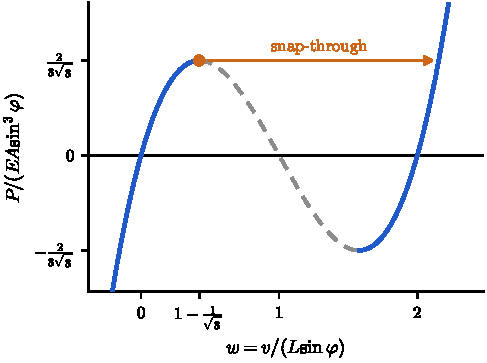
\includegraphics{ch01_bifurcation/figures/st_vonmises.pdf}
  \end{minipage}
  \caption{The von Mises truss. Left: two bars pinned at the apex under a vertical
    load; dashed, the inverted position after snap-through. Right: load against the
    symmetric deflection~\eqref{eq:st-vonmises}. The load reaches a maximum at a fold,
    and the truss jumps to the inverted branch. Solid: stable. Dashed: unstable.}
  \label{fig:st-vonmises}
\end{figure}

The maximum load is also the edge of a cliff, and the deflection gives little
warning: at $90\%$ of $p_{\max}$ the apex has moved by $w = 0.28$ only, two thirds
of the way to the fold. The warning is in the recovery time $1/f'$, here
$1/g'(w)$, which is $1.8$ at $90\%$ of $p_{\max}$, $6.0$ at $99\%$, and grows
without limit at the fold. With $z = w - 1$ the right-hand side
of~\eqref{eq:st-vonmises} is $z^3 - z$: the truss is the S-shaped curve of
Figure~\ref{fig:st-hysteresis}, and Section~\ref{sec:st-energy} explains its
hysteresis loop. Chapter~\ref{ch:ld} lets the apex move sideways as well.

%======================================================================
\section{The Hopf bifurcation: an oscillation is born}\label{sec:st-hopf}
\index{bifurcation!Hopf}%

The fold, the transcritical and the pitchfork are the three ways a real eigenvalue
can pass through zero. The fourth generic bifurcation is the other edge of
Figure~\ref{fig:st-tracedet}: a complex pair $\alpha(r) \pm i\omega$ crosses the
imaginary axis. The Jacobian stays invertible, the steady state survives, and no
new steady state appears. What appears is a periodic motion, a \emph{limit cycle}.
\index{limit cycle}%

\paragraph{The normal form.}
Two unknowns $(x,y)$ are combined into one complex number $z = x + iy$. The
normal form of the Hopf bifurcation is
\begin{equation}\label{eq:st-hopf}
  \dot z = (r + i\omega)\,z + \ell_1\,\abs{z}^2\,z ,
\end{equation}
with a real coefficient $\ell_1$. (An imaginary part of the cubic coefficient only
changes the frequency with the amplitude, and we leave it out.) The linear part has
the eigenvalues $r \pm i\omega$, which cross the imaginary axis at $r = 0$. Write
$z = \rho\,e^{i\varphi}$. Then $\dot z = (\dot\rho + i\rho\dot\varphi)\,e^{i\varphi}$,
and the real and imaginary parts of~\eqref{eq:st-hopf} separate:
\begin{equation}\label{eq:st-hopfpolar}
  \dot\rho = r\,\rho + \ell_1\,\rho^3 , \qquad \dot\varphi = \omega .
\end{equation}
The angle turns at the constant rate $\omega$. The amplitude $\rho \ge 0$ obeys a
pitchfork. If $\ell_1 < 0$, then for $r > 0$ the origin is unstable and every
motion spirals onto the circle $\rho = \sqrt{-r/\ell_1}$, traveled with the period
$2\pi/\omega$ (Figure~\ref{fig:st-hopf}). The bifurcation is
\emph{supercritical}: a small stable oscillation grows like the square root of
$r$. If $\ell_1 > 0$, an unstable cycle exists for $r < 0$ and shrinks onto the
origin at $r = 0$. After that nothing small and stable is left, and the motion jumps
to a large oscillation: the \emph{subcritical} case
(Exercise~\ref{exo:st-subhopf}).

\begin{figure}[ht]
  \centering
  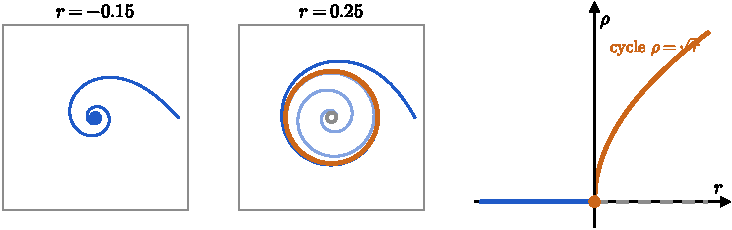
\includegraphics{ch01_bifurcation/figures/st_hopf.pdf}
  \caption{The supercritical Hopf bifurcation~\eqref{eq:st-hopf} with $\omega = 1$,
    $\ell_1 = -1$. Left: for $r < 0$ motions spiral into the origin. Middle: for
    $r > 0$ they spiral out of the origin, or in from outside, onto the limit cycle
    (orange). Right: amplitude of the cycle against $r$.}
  \label{fig:st-hopf}
\end{figure}

\begin{gbox}{When a complex pair crosses the imaginary axis, an oscillation is born}\label{sec:st-hopfthm}
\index{bifurcation!Hopf}\index{first Lyapunov coefficient}%
Suppose that at $r = r_0$ the Jacobian has one pair of eigenvalues
$\pm i\omega$, $\omega \neq 0$, all other eigenvalues having negative real parts,
that the pair crosses with nonzero speed ($d\,\mathrm{Re}\,\lambda/dr \neq 0$), and
that the \emph{first Lyapunov coefficient} $\ell_1$ is not zero. Then near
$r_0$ the system behaves like~\eqref{eq:st-hopf}: a periodic motion of period close
to $2\pi/\omega$ and amplitude proportional to $\sqrt{\abs{r - r_0}}$ is born. It is
stable when $\ell_1 < 0$.
\end{gbox}

\paragraph{Why it works.}
Look at the phase plane. Before the crossing, motions spiral inward; after, they
spiral outward. The cubic term brakes the outward spiral, and the cycle sits at the
amplitude where the linear growth $r\rho$ balances the cubic loss $\ell_1\rho^3$.
To compute $\ell_1$, bring the system at $r = r_0$ to the form
$\dot x = -\omega y + F(x,y)$, $\dot y = \omega x + G(x,y)$, where $F$ and $G$ start
with quadratic terms. Then~\cite[Section~3.4]{st-guckenheimer1983}
\begin{equation}\label{eq:st-l1}
\begin{aligned}
  16\,\ell_1 = {}& F_{xxx} + F_{xyy} + G_{xxy} + G_{yyy} \\
  &+ \frac{1}{\omega}\bigl[F_{xy}(F_{xx} + F_{yy}) - G_{xy}(G_{xx} + G_{yy})
     - F_{xx}G_{xx} + F_{yy}G_{yy}\bigr],
\end{aligned}
\end{equation}
all derivatives at the origin. The formula is long but mechanical: Mathematica
evaluates it in one line (Exercise~\ref{exo:st-computer-normal}). The theorem goes
back to Poincaré and Andronov in the plane, and to Hopf~\cite{st-hopf1942} in any
dimension.

\begin{example}[Galloping of a square prism in the wind]\label{ex:st-galloping}
\index{galloping}%
Iced power lines, bridge hangers and slender members of square section can oscillate
across the wind with large amplitudes. Den Hartog~\cite{st-denhartog1932} explained
the phenomenon for iced conductors. In a quasi-steady model, a prism of side $d$,
mass $m$ per unit length, natural frequency $\omega$ and damping ratio $\zeta$ moves
across a wind of speed $U$ with the velocity $\dot x$. It sees the wind under the
angle $\alpha \approx \dot x/U$, and the air pushes it across the wind with the force
$\tfrac12\rho_a U^2 d\,C_y(\alpha)$ per unit length, where $\rho_a$ is the air
density and $C_y = a_1\alpha - a_3\alpha^3$. For a square section
$a_1 = 2.69$ and $a_3 = 168$~\cite{st-parkinson1964}. Dividing by $m$,
\begin{equation}\label{eq:st-galloping}
  \ddot x + \omega^2 x = \gamma\,\dot x - \beta\,\dot x^3,
  \qquad
  \gamma = \frac{\rho_a d\,a_1 U}{2m} - 2\zeta\omega,
  \quad
  \beta = \frac{\rho_a d\,a_3}{2mU}.
\end{equation}
For the state $(x,\dot x)$ the Jacobian at rest is
$\begin{bmatrix} 0 & 1\\ -\omega^2 & \gamma\end{bmatrix}$, with $\det\mat{J} = \omega^2$
and $\tr\mat{J} = \gamma$. The air acts as a negative damping (this is Den Hartog's
criterion $a_1 > 0$), and it wins over the structural damping when $\gamma > 0$,
that is above the critical wind speed
\begin{equation}\label{eq:st-galloping-uc}
  U_c = \frac{4m\zeta\omega}{\rho_a\,d\,a_1}.
\end{equation}
With $y = -\dot x/\omega$, the system at $U = U_c$ has $F = 0$ and
$G = -\beta\omega^2 y^3$, so~\eqref{eq:st-l1} gives
$\ell_1 = -\tfrac38\beta\omega^2 < 0$: the Hopf bifurcation is supercritical. The
real part of the eigenvalues is $\gamma/2$, and the amplitude equation
$\dot\rho = \tfrac12\gamma\rho - \tfrac38\beta\omega^2\rho^3$ gives the amplitude
of the galloping motion,
\begin{equation}\label{eq:st-galloping-amp}
  A = \sqrt{\frac{4\gamma}{3\beta\omega^2}} .
\end{equation}
With $\rho_a = 1.25$~kg/m$^3$, $d = 0.1$~m, $m = 10$~kg/m, a frequency of
$2$~Hz ($\omega = 12.6$~rad/s) and $\zeta = 0.005$, the critical speed is
$U_c = 7.5$~m/s. At $U = 1.5\,U_c$ the amplitude is $A = 0.075$~m, three quarters
of the side; a direct integration of~\eqref{eq:st-galloping} gives the same value
(Exercise~\ref{exo:st-galloping}). Below $U_c$ nothing happens; above, the
amplitude grows like $\sqrt{U - U_c}$. Since $U_c$ is proportional to $\zeta$,
added damping is the usual cure.
\end{example}

Flutter of aircraft wings and of bridge decks is the same loss of stability with two
coupled degrees of freedom. Ziegler's column, loaded by a follower force, shows it in
a structure (Chapter~\ref{ch:ld}).

%======================================================================
\section{Potential energy, buckling and imperfections}\label{sec:st-energy}
\index{potential energy}%

\paragraph{A ball in a valley.}
Every equation $\dot y = f(y)$ in one dimension can be written
\begin{equation}\label{eq:st-gradient}
  \dot y = -\frac{dV}{dy},
\end{equation}
where the potential $V$ is an antiderivative of $-f$. Picture a ball rolling in
thick honey on the graph of $V$: it always moves downhill and never overshoots.
Steady states are the flat points of $V$. Valleys are stable, hilltops unstable,
and the slope test $f_y < 0$ is the condition $V'' > 0$. For the pitchfork,
\begin{equation}\label{eq:st-potential}
  V(y) = -\frac{r}{2}\,y^2 + \frac14\,y^4 .
\end{equation}
For $r < 0$ there is one valley. At $r = 0$ its bottom is flat to second order:
critical slowing down, seen geometrically. For $r > 0$ the bottom bulges into a
hill between two new valleys at $\pm\sqrt r$ (Figure~\ref{fig:st-potential}).

\begin{figure}[ht]
  \centering
  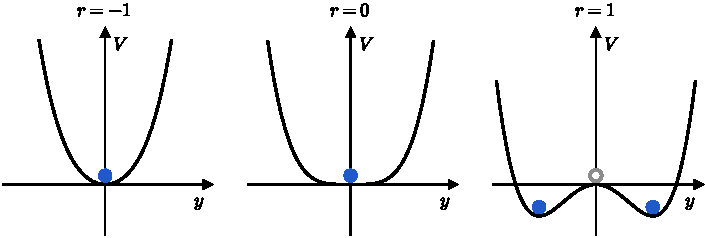
\includegraphics{ch01_bifurcation/figures/st_potential.pdf}
  \caption{The potential $V(y) = -\tfrac r2 y^2 + \tfrac14 y^4$. As $r$ passes
    through zero, one valley becomes a hill between two valleys.}
  \label{fig:st-potential}
\end{figure}

\begin{example}[The rigid bar on a torsional spring]\label{ex:st-bar}
\index{buckling!rigid bar model}%
A rigid bar of length $L$ stands on a pin. A torsional spring of stiffness $k$
holds it vertical, and a vertical dead load $P$ presses on its top
(Figure~\ref{fig:st-bar}). The rotation from the vertical is $\theta$. The spring
stores $\tfrac12 k\theta^2$, and the load descends by $L(1 - \cos\theta)$, so the
potential energy is
\begin{equation}\label{eq:st-bar-energy}
  V(\theta) = \frac12\,k\,\theta^2 - P L\,(1 - \cos\theta) .
\end{equation}
Add a rotational damper of coefficient $c$ and neglect inertia. The motion is
$c\,\dot\theta = -V'(\theta) = -k\theta + PL\sin\theta$, the gradient
form~\eqref{eq:st-gradient}. Expand $\sin\theta = \theta - \theta^3/6 + \dots$:
\begin{equation}\label{eq:st-bar-pitchfork}
  c\,\dot\theta = (PL - k)\,\theta - \frac{PL}{6}\,\theta^3 + O(\theta^5).
\end{equation}
This is the pitchfork~\eqref{eq:st-pitchfork}, with the control parameter
$r = (PL - k)/c$. The straight bar loses stability at the \emph{critical load}
$P_c = k/L$, where $f_\theta = (PL - k)/c$ passes through zero.
\index{critical load}%

Beyond $P_c$ the equilibria are exact: $k\theta = PL\sin\theta$ gives the
post-buckling path
\begin{equation}\label{eq:st-bar-path}
  \frac{P}{P_c} = \frac{\theta}{\sin\theta} \approx 1 + \frac{\theta^2}{6},
  \qquad\text{so}\qquad
  \theta \approx \pm\sqrt{6\,\frac{P - P_c}{P_c}} .
\end{equation}
The rotation grows like the square root of the excess load. On this path
$V'' = k - PL\cos\theta = k\,(1 - \theta/\tan\theta) > 0$ for
$0 < \abs\theta < \pi$: the buckled bar is stable and needs a growing load to
deflect further.
\end{example}

\begin{figure}[ht]
  \centering
  \begin{minipage}[b]{0.30\textwidth}
    \centering
    \begin{tikzpicture}[scale=0.95,>=Stealth]
      \fill[pattern=north east lines] (-0.9,-0.22) rectangle (0.9,0);
      \draw[thick] (-0.9,0) -- (0.9,0);
      \draw[gray!60,dashed] (0,0) -- (0,3.3);
      \draw[thick,domain=0:700,samples=90,smooth,variable=\t]
        plot ({(0.07+0.00028*\t)*cos(\t)},{0.25+(0.07+0.00028*\t)*sin(\t)});
      \draw[line width=2.2pt,cu] (0,0.25) -- ({3*sin(20)},{0.25+3*cos(20)});
      \fill (0,0.25) circle (1.6pt);
      \draw[->,line width=1.1pt,cphi] ({3*sin(20)},{1.35+3*cos(20)}) -- ({3*sin(20)},{0.35+3*cos(20)});
      \node[cphi,right] at ({3*sin(20)+0.05},{1.05+3*cos(20)}) {$P$};
      \draw[->] (0,1.5) arc (90:70:1.25);
      \node at (0.24,1.75) {$\theta$};
      \node[right] at (0.62,1.25) {$L$};
      \node[left] at (-0.35,0.3) {$k$};
    \end{tikzpicture}
  \end{minipage}\hfill
  \begin{minipage}[b]{0.68\textwidth}
    \centering
    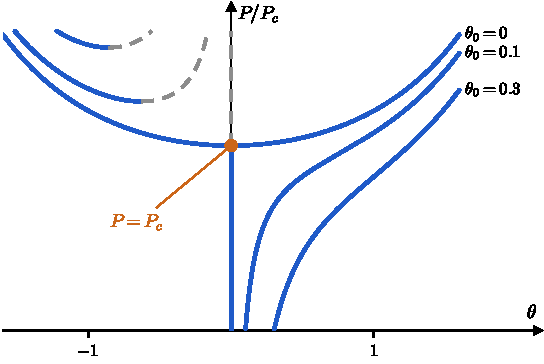
\includegraphics{ch01_bifurcation/figures/st_bar_paths.pdf}
  \end{minipage}
  \caption{Left: rigid bar on a torsional spring under a dead load. Right:
    equilibrium paths. The perfect bar ($\theta_0 = 0$) follows the pitchfork; an
    initial tilt $\theta_0$ turns it into one smooth path and a separate branch
    with a fold. Solid: stable. Dashed: unstable.}
  \label{fig:st-bar}
\end{figure}

\paragraph{Real structures are never perfect.}
\index{imperfection}%
No bar is perfectly vertical and no load perfectly centred. Give the bar an
initial tilt $\theta_0$: the spring is unloaded at $\theta = \theta_0$, the energy
becomes $\tfrac12 k(\theta - \theta_0)^2 - PL(1 - \cos\theta)$, and the equilibria
are $P/P_c = (\theta - \theta_0)/\sin\theta$. Figure~\ref{fig:st-bar} shows what
happens. The straight state is gone. The bar starts to rotate as soon as it is
loaded, smoothly and toward the side of the tilt. The pitchfork has broken into one
smooth path and a separate pair of branches that meet at a fold.

The same unfolding is seen on the normal form. Add a small constant $h$
to~\eqref{eq:st-pitchfork}:
\begin{equation}\label{eq:st-imperfect}
  \dot y = h + r\,y - y^3 .
\end{equation}
Box~\ref{sec:st-box-bif} gives the folds: $f = 0$ and $f_y = r - 3y^2 = 0$. Then
$y^2 = r/3$, and substituting in $f = 0$ gives $h = y^3 - ry = -2y^3$, so
\begin{equation}\label{eq:st-cusp}
  \abs{h} = h_c(r) = \frac{2}{3\sqrt3}\;r^{3/2}.
\end{equation}
There are three steady states for $\abs h < h_c(r)$ and one for $\abs h > h_c(r)$.
In the $(r,h)$ plane the boundary has a sharp point at the origin, a \emph{cusp}.
\index{cusp}%

\paragraph{Hysteresis.}
\index{hysteresis}%
Fix $r = 1$ and use $h$ as the control. The steady states lie on the S-shaped
curve $h = y^3 - y$ (Figure~\ref{fig:st-hysteresis}). Its folds are at
$y = \pm 1/\sqrt3$, where $h = \mp h_c$ with $h_c = 2/(3\sqrt3) \approx 0.385$.
The outer parts of the S are stable, the middle part is unstable. Sweep $h$ up
slowly from $-1$: the system follows the lower branch until it folds away at
$h = h_c$, and then jumps to the upper branch. Sweep back down: the system stays
on the upper branch until $h = -h_c$, far below the point where it jumped up, and
only then jumps down. The way up and the way down differ, and the system
remembers where it came from.
Exercise~\ref{exo:st-computer-hysteresis} reproduces the loop numerically.

\begin{figure}[ht]
  \centering
  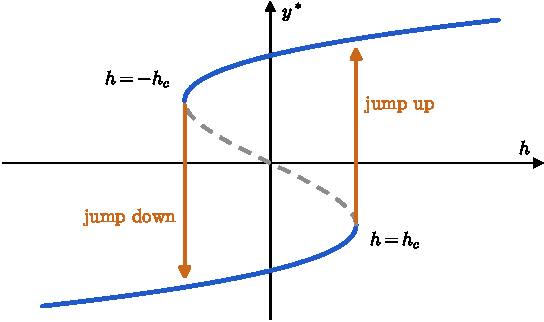
\includegraphics{ch01_bifurcation/figures/st_hysteresis.pdf}
  \caption{Steady states of $\dot y = h + y - y^3$ ($r = 1$) as the imperfection $h$
    varies. Sweeping $h$ up and down traces a hysteresis loop with jumps at the
    folds $h = \pm h_c$.}
  \label{fig:st-hysteresis}
\end{figure}

\begin{gbox}{A pitchfork needs a symmetry; without it, the saddle-node takes over}\label{sec:st-imperfection}
\index{imperfection}%
A small imperfection splits the pitchfork into one smooth branch and a pair of
saddle-nodes. The perfect system is the exception; jumps at folds and hysteresis
are what is observed.
\end{gbox}

\paragraph{Why it works.}
At a pitchfork, $f$, $f_y$, $f_r$ and $f_{yy}$ all vanish together. That is four
conditions on two unknowns $(y,r)$, possible only because the symmetry $y \to -y$
makes $f$ odd in $y$. A small $h$ destroys the symmetry. Only the two conditions
$f = f_y = 0$ of Section~\ref{sec:st-ift} remain, and their generic solutions are
folds: the two points~\eqref{eq:st-cusp}. The bar of Figure~\ref{fig:st-bar}
shows the mechanical consequence, studied in depth for elastic structures
in~\cite{st-thompson1973}. Chapter~\ref{ch:ld} measures it: how much an
imperfection lowers the largest load a structure can carry.

%======================================================================
\section{Following branches: the ideas of continuation}\label{sec:st-continuation}
\index{continuation}%

Closed forms are rare. To draw the bifurcation diagram of a real structure we
compute its branches point by point, each point starting from the previous one.
This is \emph{continuation}. The ideas are clearest on one equation $f(y,r) = 0$
for the steady states; Chapter~\ref{ch:nc} applies them to finite element models
with thousands of unknowns; the mathematics is in~\cite{st-allgower2003}.
There are two lessons. Newton's method fails at a fold,
because it divides by $f_y = 0$. Treating $r$ as an unknown repairs it.

\paragraph{Natural parameter continuation.}
\index{continuation!natural parameter}%
Suppose $(y_k,r_k)$ is a steady state. Choose the next value $r_{k+1} = r_k + \Delta r$.
The slope~\eqref{eq:st-ift} predicts $y^0 = y_k - (f_r/f_y)\,\Delta r$, and Newton's
method corrects it:
\begin{equation}\label{eq:st-newton}
  y \leftarrow y - \frac{f(y,r_{k+1})}{f_y(y,r_{k+1})}
\end{equation}
until $f = 0$. Every step divides by $f_y$, and near a fold $f_y \to 0$.
Figure~\ref{fig:st-continuation} shows the result on the S-curve
$f = h + y - y^3$ of Section~\ref{sec:st-energy}, with $h$ as the parameter. Steps
of $\Delta h = 0.08$ follow the lower branch up to the fold at $h_c = 0.385$. Past
the fold there is no solution nearby: Newton's method fails twice, and then lands
on the upper branch. The computation jumps, like the physical system, and never
sees the unstable middle branch. Two things went wrong: we divided by $f_y = 0$,
and we insisted on marching forward in $h$ while the branch turns back.

\paragraph{Pseudo-arclength continuation.}
\index{continuation!pseudo-arclength}%
Keller's idea~\cite{st-keller1977} is to make $r$ an unknown too. Write
$\mat{u} = (y,r)$. One equation $f(\mat{u}) = 0$ for two unknowns has a curve of
solutions, and we measure along it the arclength $s$. Its unit tangent
$\mat{t} = (y',r')$, with $' = d/ds$, satisfies $f_y y' + f_r r' = 0$ and
$y'^2 + r'^2 = 1$:
\begin{equation}\label{eq:st-tangent}
  \mat{t} = \frac{(-f_r,\; f_y)}{\sqrt{f_y^2 + f_r^2}} .
\end{equation}
It is the gradient $(f_y,f_r)$ turned by a right angle. At a fold, $r' = 0$ and the
tangent is vertical, but nothing else happens to it. A step goes as follows. The
predictor moves along the tangent, $\mat{u}^0 = \mat{u}_k + \Delta s\,\mat{t}_k$. The
corrector solves two equations, the second one fixing the distance travelled along
the old tangent:
\begin{equation}\label{eq:st-augmented}
  f(y,r) = 0, \qquad \mat{t}_k \cdot (\mat{u} - \mat{u}_k) - \Delta s = 0 .
\end{equation}
Newton's method for this system uses the \emph{augmented Jacobian}
\index{augmented Jacobian}%
\begin{equation}\label{eq:st-jhat}
  \widehat{\mat{J}} = \begin{bmatrix} f_y & f_r \\ y'_k & r'_k \end{bmatrix}.
\end{equation}

\begin{gbox}{The augmented Jacobian stays invertible at a fold; it is singular at a branch point}\label{sec:st-augmented}
\index{augmented Jacobian}%
On the curve, with the tangent~\eqref{eq:st-tangent},
\begin{equation}\label{eq:st-detjhat}
  \det\widehat{\mat{J}} = f_y\,r' - f_r\,y'
  = \frac{f_y^2 + f_r^2}{\sqrt{f_y^2 + f_r^2}} = \sqrt{f_y^2 + f_r^2} .
\end{equation}
At a fold $f_y = 0$ but $f_r \neq 0$: $\widehat{\mat{J}}$ is invertible and Newton's
method converges. At a transcritical or pitchfork point $f_y = f_r = 0$:
$\widehat{\mat{J}}$ is singular.
\end{gbox}

\paragraph{Why it works.}
Newton's method with $r$ fixed looks for the crossing of the curve with a vertical
line, and at a fold that line is tangent to the curve. The augmented system looks
for the crossing with a line perpendicular to the old tangent, and such a line cuts
the curve cleanly, unless the curve has no single tangent: that happens only where
two branches cross. With $n$ unknowns,
$\widehat{\mat{J}} = \begin{bmatrix} \mat{J} & \mat{f}_r \\ \mat{t}_y\T & t_r\end{bmatrix}$
is $(n+1)\times(n+1)$, and it is singular exactly when the $n\times(n+1)$ matrix
$\begin{bmatrix}\mat{J} & \mat{f}_r\end{bmatrix}$ loses rank. At a fold the zero
eigenvalue of $\mat{J}$ comes with $\mat{w}\T\mat{f}_r \neq 0$
(Section~\ref{sec:st-zero}), the column $\mat{f}_r$ makes up for the lost rank, and
$\widehat{\mat{J}}$ is invertible. At a branch point $\mat{w}\T\mat{f}_r = 0$ and it is
not. The eigenvalue problem $\mat{J}\mat{v} = \mat{0}$, with its left eigenvector
$\mat{w}$, tells everything: where the plain Newton method breaks down, in which
direction $\mat{v}$ the branch turns or splits, and whether the augmented method
goes through.

\paragraph{The implicit function theorem behind each step.}
\index{implicit function theorem}%
The corrector solves $\mat{F}(\mat{u},s) = \mat{0}$, with
\[
  \mat{F}(\mat{u},s) = \begin{bmatrix} \mat{f}(\mat{u}) \\
  \mat{t}_k\cdot(\mat{u} - \mat{u}_k) - s \end{bmatrix}.
\]
These are $n+1$ equations for the $n+1$ unknowns $\mat{u} = (\mat{y},r)$, and the
arclength $s$ plays the part of the parameter. The Jacobian of $\mat{F}$ with respect to
$\mat{u}$ is $\widehat{\mat{J}}$. So wherever $\widehat{\mat{J}}$ is invertible,
Section~\ref{sec:st-iftn} applies with $\mat{u}$ in place of $\mat{y}$ and $s$ in place
of $r$: near $\mat{u}_k$ there is exactly one smooth solution $\mat{u}^*(s)$, and for a
small enough $\Delta s$ the Newton corrector converges to it. Natural parameter
continuation applies the same theorem with $r$ as the parameter, and needs
$\mat{J}$ invertible; it breaks down at the fold of Figure~\ref{fig:st-ift}. The
arclength is a parameter that the curve chooses itself, along its own tangent, and
it breaks down only at the branch point, where no parameter can work.

\begin{gbox}{Box 1.2\quad Pseudo-arclength continuation of $\mat{f}(\mat{y},r) = \mat{0}$}\label{sec:st-box-arc}
\index{continuation!pseudo-arclength}%
Unknowns $\mat{u} = (\mat{y},r)$. Given a solution $\mat{u}_0$, a step $\Delta s$, and a
rough direction $\mat{t}_{\mathrm{old}}$.
\begin{enumerate}[label=\arabic*.]
  \item Tangent: solve
        $\begin{bmatrix}\mat{J} & \mat{f}_r\\ \mat{t}_{\mathrm{old}}\T\end{bmatrix}\mat{t}
        = \begin{bmatrix}\mat{0}\\ 1\end{bmatrix}$ at $\mat{u}_k$, and normalize
        $\mat{t}_k = \mat{t}/\abs{\mat{t}}$. The last row keeps the direction of travel.
  \item Predictor: $\mat{u} = \mat{u}_k + \Delta s\,\mat{t}_k$.
  \item Corrector: repeat
        $\widehat{\mat{J}}\,\delta\mat{u} = -\begin{bmatrix}\mat{f}(\mat{u})\\
        \mat{t}_k\cdot(\mat{u} - \mat{u}_k) - \Delta s\end{bmatrix}$,
        $\mat{u} \leftarrow \mat{u} + \delta\mat{u}$, until $\abs{\delta\mat{u}}$ is
        small. If it does not converge, halve $\Delta s$ and return to step~2.
  \item Monitor, between $\mat{u}_k$ and $\mat{u}_{k+1}$, the signs of $r'$ (folds),
        of $\det\mat{J}$ (an eigenvalue through zero: folds and branch points) and of
        $\det\widehat{\mat{J}}$ (branch points).
  \item Set $\mat{t}_{\mathrm{old}} = \mat{t}_k$, $k \leftarrow k+1$, and return to
        step~1.
\end{enumerate}
\end{gbox}

\begin{figure}[ht]
  \centering
  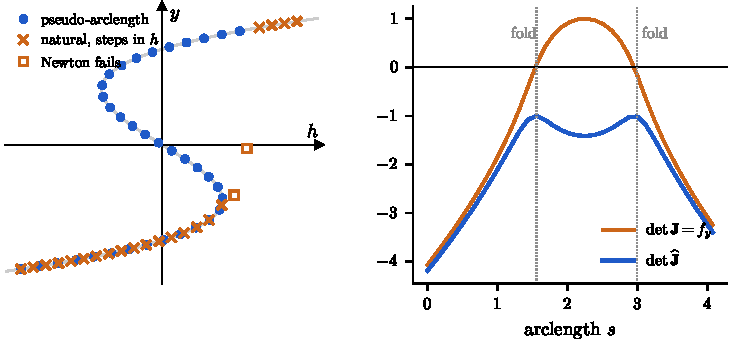
\includegraphics{ch01_bifurcation/figures/st_continuation.pdf}
  \caption{The S-curve $h + y - y^3 = 0$. Left: steps in $h$ (natural parameter) jump
    at the fold; pseudo-arclength steps ($\Delta s = 0.12$) go round both folds.
    Right: along the pseudo-arclength path, $\det\mat{J} = f_y$ changes sign at each
    fold, while $\det\widehat{\mat{J}}$ never vanishes.}
  \label{fig:st-continuation}
\end{figure}

\paragraph{Detecting and switching.}
\index{branch switching}%
The monitors of step~4 change sign between two points, and a linear interpolation
locates the zero (Figure~\ref{fig:st-continuation}, right). On the S-curve,
$\det\mat{J}$ changes sign at both folds and $\det\widehat{\mat{J}}$ keeps its sign. On
the straight state $\theta = 0$ of the perfect bar, written $\theta - p\sin\theta = 0$
with $p = P/P_c$, the tangent is $(0,1)$ and $\det\widehat{\mat{J}} = f_\theta = 1 - p$
changes sign at $p = 1$: a branch point. To leave it on the new branch we need the
directions $(a,b)$ of the branches through the point. The second-order terms
of~\eqref{eq:st-taylor} give them:
$f_{yy}a^2 + 2f_{yr}\,ab + f_{rr}b^2 = 0$. At a pitchfork this reduces to $ab = 0$:
the old branch $(0,1)$ and the new one $(1,0)$, at a right angle. A small step in
the new direction, followed by the corrector, puts the computation on the buckled
branch.

\paragraph{What the code finds.}
Exercise~\ref{exo:st-computer-arclength} writes Box~1.2 in about fifty lines of Python.
With $\Delta s = 0.05$ it locates the folds of the S-curve at $h = \pm0.384$
(exact: $\pm0.3849$). For the bar with a tilt $\theta_0 = 0.1$ it finds the fold
of the complementary branch at $\theta = -0.632$, $P/P_c = 1.239$. On the perfect
bar it detects the branch point at $P = P_c$ and follows the buckled branch,
$P/P_c = \theta/\sin\theta$, to machine precision. In Chapter~\ref{ch:nc} the scalar
$f_y$ becomes the tangent stiffness matrix of a finite element model, $\mat{f}_r$ the
load vector, and Box~1.2 becomes the arc-length methods of Riks and Crisfield. A
zero eigenvalue of the tangent stiffness, $\mat{J}\mat{v} = \mat{0}$, is a buckling
load, and linear buckling analysis is this eigenvalue problem.

%======================================================================
\framepart{Summary}
\begin{gbox*}
\begin{itemize}
  \item \textbf{Steady states and stability.} A steady state solves $f(y^*,r) = 0$.
        It is stable when $\lambda = f_y(y^*,r) < 0$, and disturbances then die out
        in a time of about $1/\abs\lambda$.
  \item \textbf{Lyapunov.} A function with a minimum at $y^*$ that never increases
        along the motion proves stability, even where the slope test is silent.
        In mechanics the energy is that function.
  \item \textbf{Several unknowns.} The eigenvalues of the Jacobian $\mat{J}$ are the
        growth rates. Stability is lost when a real eigenvalue crosses zero
        (divergence, buckling) or a complex pair crosses the imaginary axis
        (flutter, galloping).
  \item \textbf{Linear is not enough.} $\dot y = ay$ has a single steady state.
        Several steady states need a nonlinear $f$ whose graph bends.
  \item \textbf{Where bifurcations happen.} While $f_y \neq 0$ (with $n$ unknowns,
        $\det\mat{J} \neq 0$) the steady state is unique and moves smoothly with $r$:
        this is the implicit function theorem. New states can appear only where
        $f = 0$ and $f_y = 0$ together.
  \item \textbf{One number, two jobs.} $f_y$ controls stability and uniqueness.
        When the control parameter drives $\lambda$ through zero, stability is lost
        and new solutions can appear.
  \item \textbf{Four generic bifurcations.} Fold (saddle-node) $r + y^2$,
        transcritical $ry - y^2$, pitchfork $ry \mp y^3$, and Hopf
        $\dot z = (r + i\omega)z + \ell_1\abs{z}^2z$. The Taylor coefficients $f_r$,
        $f_{yy}$, $f_{yr}$, $f_{yyy}$ (and $\ell_1$ for Hopf) tell which, and whether
        it is super- or subcritical.
  \item \textbf{Zero eigenvalue.} New branches appear only where
        $\mat{J}\mat{v} = \mat{0}$. With the left eigenvector $\mat{w}$:
        fold if $\mat{w}\T\mat{f}_r \neq 0$, branch point if $\mat{w}\T\mat{f}_r = 0$.
  \item \textbf{Buckling.} The rigid bar on a spring buckles at $P_c = k/L$ through
        a pitchfork, with $\theta \approx \pm\sqrt{6(P - P_c)/P_c}$.
  \item \textbf{Warning signs.} Slow recovery from disturbances (critical slowing
        down), and with imperfections, jumps at folds and hysteresis.
  \item \textbf{Continuation.} Stepping in the parameter fails at a fold, where
        $f_y = 0$. Pseudo-arclength continuation makes the parameter an unknown; its
        augmented Jacobian stays invertible at folds and becomes singular only at
        branch points, where the branch is switched. Each step is the implicit
        function theorem with the arclength as the parameter.
\end{itemize}
\end{gbox*}

%======================================================================
\framepart{Exercises}\label{sec:st-exo}

\framesub{Short questions}

\exercise{Three steady states}\label{exo:st-three}
\index{stability}%
Find the steady states of $\dot y = y(1-y)(y-2)$ and their stability, first from
the phase line, then from $f'(y^*)$.
\begin{solution}
The steady states are $0$, $1$, $2$. Expanding, $f = -y^3 + 3y^2 - 2y$ and
$f' = -3y^2 + 6y - 2$. Then $f'(0) = -2$ (stable), $f'(1) = 1$ (unstable),
$f'(2) = -2$ (stable). The phase line agrees: $f < 0$ on $(0,1)$ and $f > 0$ on
$(1,2)$, so the arrows leave $1$ and point to $0$ and $2$.
\end{solution}

\exercise{Slow decay}\label{exo:st-slow}
\index{critical slowing down}%
With $y(0) = 1$, how long does $\dot y = -y^3$ take to reach $y = \tfrac12$?
Compare with $\dot y = -y$.
\begin{solution}
From~\eqref{eq:st-slowdecay}, $1/y^2 = 1 + 2t$, so $4 = 1 + 2t$ and $t = 1.5$. For
$\dot y = -y$, $e^{-t} = \tfrac12$ gives $t = \ln 2 \approx 0.69$. The cubic is
already twice slower over the first halving, and the gap widens: reaching
$y = 0.01$ takes $5000$ time units instead of $4.6$.
\end{solution}

\exercise{When the slope test is silent}\label{exo:st-silent}
Draw the phase lines of $\dot y = -y^3$, $\dot y = y^3$ and $\dot y = y^2$ near
$y = 0$. Which is stable?
\begin{solution}
$-y^3$: arrows point toward $0$ from both sides, stable. $y^3$: arrows point away
on both sides, unstable. $y^2 \ge 0$: arrows point right on both sides, so $0$
attracts from the left and repels to the right (semi-stable). All three have
$f'(0) = 0$.
\end{solution}

\exercise{A saddle-node in disguise}\label{exo:st-disguise}
\index{bifurcation!saddle-node}%
Find the bifurcation points of $\dot y = r - y - e^{-y}$ and their type.
\begin{solution}
$f_y = -1 + e^{-y} = 0$ gives $y = 0$, and then $f = 0$ gives $r = 1$. The function
$g(y) = y + e^{-y}$ has its minimum $1$ at $y = 0$, so $f = r - g(y) = 0$ has two
roots for $r > 1$ and none for $r < 1$: a saddle-node at $(y,r) = (0,1)$, with
$f_r = 1 \neq 0$. The root with $y > 0$ is stable ($f_y < 0$).
\end{solution}

\exercise{Which way does it open?}\label{exo:st-open}
Draw the bifurcation diagram of $\dot y = r - y^2$ and compare with
Figure~\ref{fig:st-normalforms}.
\begin{solution}
Steady states $\pm\sqrt r$ for $r > 0$, none for $r < 0$. With $f_y = -2y$,
$+\sqrt r$ is stable and $-\sqrt r$ unstable. The parabola opens to the right,
the mirror image of $r + y^2$.
\end{solution}

\exercise{A Lyapunov function where the eigenvalues are silent}\label{exo:st-lyap}
\index{Lyapunov function}%
Consider $\ddot x + \dot x + x^3 = 0$. (a)~Write it for $(x,\dot x)$ and find the
eigenvalues of the Jacobian at the origin. (b)~Show that
$W = \tfrac12\dot x^2 + \tfrac14 x^4$ is a Lyapunov function and conclude.
\begin{solution}
(a)~$\dot x = \dot x$, $\ddot x = -\dot x - x^3$, so
$\mat{J} = \begin{bmatrix} 0 & 1\\ 0 & -1\end{bmatrix}$, with eigenvalues $0$ and $-1$:
the test of Section~\ref{sec:st-eigen} is silent (the spring has no linear part).
(b)~$\dot W = \dot x\ddot x + x^3\dot x = \dot x(-\dot x - x^3) + x^3\dot x = -\dot x^2 \le 0$,
and $W > 0$ away from the origin: stable. As for the damped oscillator, a motion
cannot stay on $\dot x = 0$ unless $x = 0$, so the origin is asymptotically stable.
The return is slow, like that of $\dot y = -y^3$.
\end{solution}

\exercise{Measuring a buckling load by vibration}\label{exo:st-tracedet}
\index{divergence}%
The bar of Section~\ref{sec:st-lyapunov} has $mL^2 = 1$~kg\,m$^2$, $L = 1$~m,
$k = 100$~N\,m/rad and $c = 2$~N\,m\,s. Find the eigenvalues at $\theta = 0$ for
$P = 0$, $75$ and $120$~N. How does the frequency depend on $P$?
\begin{solution}
$\lambda^2 + 2\lambda + (100 - P) = 0$. $P = 0$: $\lambda = -1 \pm 9.95\,i$.
$P = 75$: $\lambda = -1 \pm 4.90\,i$. $P = 120$: $\lambda = -1 \pm \sqrt{21}$, that is
$3.58$ and $-5.58$: a positive real eigenvalue, the bar diverges (buckles). In the
undamped limit $\omega^2 = (k - PL)/(mL^2)$ decreases linearly with $P$ and vanishes at
$P_c = 100$~N. Measuring the frequency at a few safe loads and extrapolating to
$\omega = 0$ gives the buckling load without reaching it. This is the idea of the
vibration correlation technique used on shells (Chapter~\ref{ch:cy}).
\end{solution}

\exercise{A limit cycle by hand}\label{exo:st-hopfshort}
\index{limit cycle}%
For $\dot\rho = r\rho - \rho^3$, $\dot\varphi = 2\pi$ with $r = 0.04$, find the
amplitude, the period and the stability of the cycle.
\begin{solution}
$\rho^2 = r$ gives $\rho = 0.2$. The period is $2\pi/\omega = 1$. The slope of
$r\rho - \rho^3$ at $\rho = 0.2$ is $r - 3\rho^2 = -2r = -0.08 < 0$: stable, with a
relaxation time of $12.5$ periods. Near the bifurcation, cycles are small and slow
to settle.
\end{solution}

\exercise{Why Newton's method stops at a fold}\label{exo:st-newton}
\index{augmented Jacobian}%
At the fold $(y,h) = (-1/\sqrt3,\, 2/(3\sqrt3))$ of $f = h + y - y^3$, compute $f_y$,
$f_h$, the tangent~\eqref{eq:st-tangent} and $\det\widehat{\mat{J}}$.
\begin{solution}
$f_y = 1 - 3y^2 = 0$ and $f_h = 1$. The tangent is $(-1, 0)$: vertical in the
$(h,y)$ plane, pure change of $y$. Newton's method in $y$ at fixed $h$ divides by
$f_y = 0$. The augmented Jacobian
$\begin{bmatrix} 0 & 1\\ -1 & 0\end{bmatrix}$ has determinant $1$: the augmented
Newton method has no difficulty.
\end{solution}

\exercise{The circle and the implicit function theorem}\label{exo:st-circle}
\index{implicit function theorem}%
For $f(y,r) = r^2 + y^2 - 1$: (a)~at which points does Section~\ref{sec:st-iftn} give
$y$ as a function of $r$, and with which slope? (b)~Where does it give $r$ as a
function of $y$? (c)~Compute $\det\widehat{\mat{J}}$ on the circle and conclude that
pseudo-arclength continuation goes round the whole circle.
\begin{solution}
(a)~Wherever $f_y = 2y \neq 0$, that is everywhere except $(\pm1,0)$, with
$dy^*/dr = -f_r/f_y = -r/y$. (b)~Wherever $f_r = 2r \neq 0$: everywhere except
$(0,\pm1)$. The two charts together cover the circle. (c)~By~\eqref{eq:st-detjhat},
$\det\widehat{\mat{J}} = \sqrt{f_y^2 + f_r^2} = 2\sqrt{r^2 + y^2} = 2$ on the circle:
never zero. The circle has two folds in $r$ (at $r = \pm1$) and none is a problem for
the arclength; there is no branch point.
\end{solution}

\framesub{Problems}

\exercise{Snap-through of the von Mises truss}\label{exo:st-vonmises}
\index{von Mises truss}\index{snap-through}%
For the truss of Example~\ref{ex:st-vonmises}:
(a)~find the steady states for $p = 0$ and their stability;
(b)~derive the maximum and minimum loads $\pm p_{\max}$;
(c)~describe what the apex does when $p$ is raised slowly to $0.5$ and then
brought back to $-0.5$.
\begin{solution}
(a)~$w = 0$ (the built shape) and $w = 2$ (the inverted shape) are stable,
since $g'(0) = g'(2) = 2 > 0$; $w = 1$ (bars horizontal) is unstable, $g'(1) = -1$.
(b)~$g'(w) = 3w^2 - 6w + 2 = 0$ at $w = 1 \mp 1/\sqrt3$, where
$g = \pm 2/(3\sqrt3)$.
(c)~The apex follows the first branch up to $p_{\max} \approx 0.385$ at
$w \approx 0.42$, jumps to $w \approx 2.15$ and continues on the inverted branch.
On the way back it stays inverted until $p = -p_{\max}$ at $w \approx 1.58$ and
jumps back to $w \approx -0.15$: a hysteresis loop, as in
Figure~\ref{fig:st-hysteresis}.
\end{solution}

\exercise{The subcritical pitchfork}\label{exo:st-subcritical}
\index{bifurcation!pitchfork}%
Study $\dot y = ry + y^3$: steady states, stability, bifurcation diagram. Why is
it more dangerous than~\eqref{eq:st-pitchfork}?
\begin{solution}
$y^* = 0$ for all $r$, and $y^* = \pm\sqrt{-r}$ for $r < 0$. The slope is
$f_y = r + 3y^2$: it equals $r$ at $0$ and $-2r > 0$ at $\pm\sqrt{-r}$. For $r < 0$
the stable origin is flanked by two unstable states, which bound its basin of
attraction and shrink to it as $r \to 0$. For $r > 0$ nothing stable is left near
$0$ and $y$ escapes to infinity in finite time. There is no gentle post-critical
state: the loss of stability is a jump. A stabilising term $-y^5$ creates two
far-away stable branches and a hysteresis loop.
\end{solution}

\exercise{The cusp}\label{exo:st-cusp}
\index{cusp}%
Derive~\eqref{eq:st-cusp}. Sketch the region of the $(r,h)$ plane where
$\dot y = h + ry - y^3$ has three steady states.
\begin{solution}
Section~\ref{sec:st-energy}. The region is
$\abs h < \tfrac{2}{3\sqrt3}\,r^{3/2}$, $r > 0$: a wedge bounded by two branches
of a semicubical parabola that meet tangentially at the origin.
\end{solution}

\exercise{The imperfect bar}\label{exo:st-imperfect-bar}
\index{buckling!rigid bar model}%
\index{imperfection}%
For the bar of Example~\ref{ex:st-bar} with an initial tilt $\theta_0 > 0$:
(a)~show that the equilibria are $P/P_c = (\theta - \theta_0)/\sin\theta$;
(b)~show that the natural path ($\theta > \theta_0$) is stable;
(c)~find the rotation when the load reaches $P_c$ and show that it scales as
$\theta_0^{1/3}$. Evaluate it for $\theta_0 = 0.01$.
\begin{solution}
(a)~$V = \tfrac12 k(\theta - \theta_0)^2 - PL(1 - \cos\theta)$ and $V' = 0$ give
$k(\theta - \theta_0) = PL\sin\theta$, with $P_c = k/L$.
(b)~$V'' = k - PL\cos\theta = k\bigl(1 - (\theta - \theta_0)/\tan\theta\bigr)$, and
$(\theta - \theta_0)/\tan\theta < \theta/\tan\theta < 1$ for $0 < \theta < \pi/2$.
(c)~$P = P_c$ gives $\theta - \sin\theta = \theta_0$, and
$\theta - \sin\theta \approx \theta^3/6$, so $\theta \approx (6\theta_0)^{1/3}$. For
$\theta_0 = 0.01$: $\theta \approx 0.39$ (the exact root is $0.392$). A tilt of
$0.6^\circ$ gives a rotation of $22^\circ$ at the critical load: the cube root
amplifies small imperfections.
\end{solution}

\exercise{The imperfect transcritical bifurcation}\label{exo:st-imptrans}
\index{bifurcation!transcritical}\index{imperfection}%
Study $\dot y = h + ry - y^2$ for small $h > 0$ and $h < 0$: steady states,
stability, folds. How far does the critical value of $r$ move?
\begin{solution}
$y_\pm = \tfrac12\bigl(r \pm \sqrt{r^2 + 4h}\bigr)$, with $f_y = r - 2y = \mp\sqrt{r^2+4h}$:
$y_+$ is stable, $y_-$ unstable. For $h > 0$ the square root is always real: two
separate branches, a hyperbola, and the exchange of stability is replaced by a smooth
passage on $y_+$. For $h < 0$ there are no steady states for $\abs r < 2\sqrt{-h}$,
and folds at $r = \pm2\sqrt{-h}$, $y = r/2$. The critical value moves by an amount
proportional to $\sqrt{\abs h}$, much more than $h$ itself. In structures this is the
one-half power law of asymmetric bifurcation (Chapter~\ref{ch:ld}).
\end{solution}

\exercise{The van der Pol oscillator}\label{exo:st-vdp}
\index{bifurcation!Hopf}%
For $\ddot x - (\mu - x^2)\dot x + x = 0$: (a)~find the eigenvalues at the origin and
the Hopf point; (b)~with $y = -\dot x$, compute $\ell_1$ by~\eqref{eq:st-l1};
(c)~deduce the amplitude of the cycle for small $\mu > 0$.
\begin{solution}
(a)~$\lambda^2 - \mu\lambda + 1 = 0$: $\lambda = \tfrac\mu2 \pm i\sqrt{1 - \mu^2/4}$.
The real part $\mu/2$ crosses zero at $\mu = 0$ with $\omega = 1$.
(b)~$\dot x = -y$, $\dot y = x + (\mu - x^2)y$. At $\mu = 0$: $F = 0$,
$G = -x^2y$, so $16\ell_1 = G_{xxy} = -2$ and $\ell_1 = -\tfrac18$: supercritical.
(c)~$\dot\rho = \tfrac\mu2\rho - \tfrac18\rho^3$ gives $\rho = 2\sqrt\mu$, the classical
amplitude of the van der Pol cycle.
\end{solution}

\exercise{The subcritical Hopf bifurcation and its hysteresis}\label{exo:st-subhopf}
\index{bifurcation!Hopf}\index{hysteresis}%
Study the cycles of $\dot\rho = r\rho + \rho^3 - \rho^5$ as $r$ increases from $-1$ to
$1$ and back.
\begin{solution}
Cycles solve $r + \rho^2 - \rho^4 = 0$: $\rho^2 = \tfrac12\bigl(1 \pm \sqrt{1 + 4r}\bigr)$,
real for $r \ge -\tfrac14$. The slope of $g(\rho) = r\rho + \rho^3 - \rho^5$ at a cycle is
$2\rho^2(1 - 2\rho^2)$: the outer cycle ($\rho^2 > \tfrac12$) is stable, the inner one
unstable. For $-\tfrac14 < r < 0$ the stable rest state, an unstable cycle and a large
stable cycle coexist. Increasing $r$: the system rests until $r = 0$, then jumps to the
cycle $\rho = 1$. Decreasing $r$: it stays on the large cycle until the fold of cycles
at $r = -\tfrac14$, $\rho = 1/\sqrt2$, then falls back to rest. Oscillations start
abruptly and stop at a lower parameter value.
\end{solution}

\exercise{Galloping}\label{exo:st-galloping}
\index{galloping}%
(a)~Derive~\eqref{eq:st-galloping-uc} and~\eqref{eq:st-galloping-amp}, the amplitude
also by an energy balance over one cycle $x = A\cos\omega t$. (b)~Evaluate $U_c$ and
$A$ at $U = 1.1$, $1.5$ and $2\,U_c$ for the data of Example~\ref{ex:st-galloping}, and
check by integrating~\eqref{eq:st-galloping}. (c)~What does doubling $\zeta$ do?
\begin{solution}
(a)~Example~\ref{ex:st-galloping}. Energy balance: the work of
$\gamma\dot x - \beta\dot x^3$ over a cycle vanishes, $\gamma\langle\dot x^2\rangle
= \beta\langle\dot x^4\rangle$, with $\langle\dot x^2\rangle = \tfrac12A^2\omega^2$ and
$\langle\dot x^4\rangle = \tfrac38A^4\omega^4$, so $A^2 = 4\gamma/(3\beta\omega^2)$.
(b)~$U_c = 7.47$~m/s. Theory and integration agree: $A = 0.0288$, $0.0753$,
$0.1229$~m. Close to $U_c$ the integration needs a long time to settle (critical
slowing down: the growth rate is $\gamma/2$).
(c)~$U_c$ doubles. At a fixed wind speed above both thresholds the amplitude drops.
\lstinputlisting[firstline=4]{ch01_bifurcation/code/python/ex_galloping.py}
\end{solution}

\exercise{Computer: settling and slowing down}\label{exo:st-computer-pitchfork}
\index{critical slowing down}%
Integrate~\eqref{eq:st-pitchfork} for $r = -0.5$, $-0.1$, $0.1$, $0.5$, $1$, from
$y_0 = \pm 0.01$, and report the final state. Then measure the time to fall from
$y = 1$ to $y = 0.1$ for $r = -1$, $-0.1$, $-0.01$, $0$.
\begin{solution}
For $r < 0$ both pushes return to $0$. For $r > 0$ the solution settles at
$\pm\sqrt r$ ($\pm 0.3162$, $\pm 0.7071$, $\pm 1$), on the side of the initial
push. The times are $1.96$, $11.51$, $34.16$ and $49.50$: they grow as $r \to 0$.
At $r = 0$, \eqref{eq:st-slowdecay} gives $100 = 1 + 2t$, so $t = 49.5$, as computed.
\lstinputlisting[firstline=4]{ch01_bifurcation/code/python/ex_pitchfork.py}
\end{solution}

\exercise{Computer: a hysteresis loop}\label{exo:st-computer-hysteresis}
\index{hysteresis}%
Integrate $\dot y = h + y - y^3$ while $h$ increases from $-1$ to $1$ in steps of
$0.005$ and then decreases back, each time starting from the previous final state.
Locate the jumps and compare with Figure~\ref{fig:st-hysteresis}.
\begin{solution}
The system jumps up between $h = 0.385$ and $0.390$, from $y = -0.578$ to
$+1.156$, and down between $h = -0.385$ and $-0.390$, from $+0.578$ to $-1.156$.
Theory: folds at $h = \pm h_c = \pm 0.385$ with $y = \mp 1/\sqrt3 = \mp 0.577$, and
landing points $\pm 2/\sqrt3 = \pm 1.155$, the other roots of
$y^3 - y \pm h_c = (y \mp 1/\sqrt3)^2(y \pm 2/\sqrt3)$.
\lstinputlisting[firstline=4]{ch01_bifurcation/code/python/ex_hysteresis.py}
\end{solution}

\exercise{Computer: pseudo-arclength continuation from scratch}\label{exo:st-computer-arclength}
\index{continuation!pseudo-arclength}%
Program Box~1.2 for $\mat{f}(\mat{u}) = \mat{0}$, $\mat{u} = (\mat{y},r)$, with the
Jacobian by finite differences. (a)~Follow the S-curve $h + y - y^3 = 0$ from
$y = -1.3$ and locate its folds. (b)~Follow the complementary branch of the bar with
tilt $\theta_0 = 0.1$, $(\theta - \theta_0) - p\sin\theta = 0$, from $\theta = -2.5$,
and locate its fold. (c)~Follow the straight state of the perfect bar, detect the
branch point, switch, and compare the buckled branch with $p = \theta/\sin\theta$.
\begin{solution}
(a)~Folds at $(y,h) = (-0.577, 0.385)$ and $(0.577,-0.384)$ (exact
$\mp1/\sqrt3$, $\pm2/(3\sqrt3)$); $\det\mat{J}$ changes sign twice, $\det\widehat{\mat{J}}$
never. (b)~$\theta = -0.632$, $p = 1.239$ (exact $-0.6317$, $1.2391$, from
$\sin\theta = (\theta - \theta_0)\cos\theta$). On this branch the bar leans against its
tilt, and it is reached only by a large disturbance. (c)~$\det\widehat{\mat{J}}$ changes
sign at $p = 1.000$; the switched branch satisfies $p = \theta/\sin\theta$ to
$10^{-16}$. The orientation row in the tangent system is what makes the sign of
$\det\widehat{\mat{J}}$ meaningful from one step to the next.
\lstinputlisting[firstline=4]{ch01_bifurcation/code/python/arclength.py}
\end{solution}

\exercise{Computer: normal forms in Mathematica}\label{exo:st-computer-normal}
\index{bifurcation!normal form}%
Write a function that takes $f(y,r)$ and a point, computes the Taylor coefficients
of Section~\ref{sec:st-reduction}, and returns the type and the scalings $R$, $Y$.
Apply it to $r - y - e^{-y}$ at $(0,1)$, to $y(1-y) - ry$ at $(0,1)$ and to the bar.
Find the cusp~\eqref{eq:st-cusp} by eliminating $y$, and compute $\ell_1$
by~\eqref{eq:st-l1} for the van der Pol and the galloping oscillators.
\begin{solution}
Fold with $R = -(r-1)/2$, $Y = -y/2$; transcritical with $R = -(r-1)$, $Y = y$;
supercritical pitchfork with $R = L(P - k/L)/c$ and $f_{\theta\theta\theta} = -k/c$.
The resultant of $f$ and $f_y$ in $y$ is $4r^3 - 27h^2$ (up to sign): the cusp
$\abs h = 2r^{3/2}/(3\sqrt3)$. $\ell_1 = -\tfrac18$ (van der Pol) and
$-\tfrac38\beta\omega^2$ (galloping). A SymPy version of the same steps gives the same
results.
\lstinputlisting[language=Mathematica,firstline=4]{ch01_bifurcation/code/mathematica/normal_forms.wl}
\end{solution}

%======================================================================
\begin{chapterbib}{99}
\bibitem{st-strang2014} G.~Strang, \emph{Differential Equations and Linear
  Algebra}, Wellesley--Cambridge Press, 2014.
\bibitem{st-strogatz2015} S.~H.~Strogatz, \emph{Nonlinear Dynamics and Chaos},
  2nd~ed., Westview Press, 2015. Chapters~2, 3 and~5--8.
\bibitem{st-guckenheimer1983} J.~Guckenheimer and P.~Holmes, \emph{Nonlinear
  Oscillations, Dynamical Systems, and Bifurcations of Vector Fields}, Springer,
  1983. Chapter~3.
\bibitem{st-rudin1976} W.~Rudin, \emph{Principles of Mathematical Analysis}, 3rd~ed.,
  McGraw-Hill, 1976. Theorems~9.24 (inverse function) and~9.28 (implicit function).
\bibitem{st-krantz2002} S.~G.~Krantz and H.~R.~Parks, \emph{The Implicit Function
  Theorem: History, Theory, and Applications}, Birkh\"auser, 2002.
\bibitem{st-kuznetsov2004} Yu.~A.~Kuznetsov, \emph{Elements of Applied Bifurcation
  Theory}, 3rd~ed., Springer, 2004.
\bibitem{st-seydel2010} R.~Seydel, \emph{Practical Bifurcation and Stability
  Analysis}, 3rd~ed., Springer, 2010.
\bibitem{st-lyapunov1992} A.~M.~Lyapunov, \emph{The General Problem of the Stability
  of Motion} (1892), translated by A.~T.~Fuller, Taylor \& Francis, 1992.
\bibitem{st-hopf1942} E.~Hopf, Abzweigung einer periodischen L\"osung von einer
  station\"aren L\"osung eines Differentialsystems, \emph{Berichte der
  Math.-Phys.\ Klasse der S\"achs.\ Akad.\ Wiss.\ Leipzig} 94 (1942) 3--22.
\bibitem{st-denhartog1932} J.~P.~Den~Hartog, Transmission line vibration due to
  sleet, \emph{Transactions of the AIEE} 51 (1932) 1074--1076.
\bibitem{st-parkinson1964} G.~V.~Parkinson and J.~D.~Smith, The square prism as an
  aeroelastic non-linear oscillator, \emph{Quarterly Journal of Mechanics and Applied
  Mathematics} 17 (1964) 225--239.
\bibitem{st-keller1977} H.~B.~Keller, Numerical solution of bifurcation and
  nonlinear eigenvalue problems, in P.~H.~Rabinowitz (ed.), \emph{Applications of
  Bifurcation Theory}, Academic Press, 1977, 359--384.
\bibitem{st-allgower2003} E.~L.~Allgower and K.~Georg, \emph{Introduction to
  Numerical Continuation Methods}, SIAM, 2003.
\bibitem{st-thompson1973} J.~M.~T.~Thompson and G.~W.~Hunt, \emph{A General
  Theory of Elastic Stability}, Wiley, 1973.
\bibitem{st-scheffer2009} M.~Scheffer, J.~Bascompte, W.~A.~Brock, V.~Brovkin,
  S.~R.~Carpenter, V.~Dakos, H.~Held, E.~H.~van~Nes, M.~Rietkerk and G.~Sugihara,
  Early-warning signals for critical transitions, \emph{Nature} 461 (2009) 53--59.
\end{chapterbib}
